

\section{Technologies}

\subsection{Frontend}
% Three languages can be used to implement the frontend while using one of the main popular frameworks. This consists of i) JavaScript \cite{javascript}, ii) TypeScript \cite{typescript} and iii) Scala.js \cite{scalajs}. We decided to avoid JavaScript due to the lack of type support. Between TypeScript and Scala.js, we ended up choosing TypeScript over Scala.js. That is because we are more familiar with TypeScript than Scala.js. Moreover, the advantages of Scala.js, according to their website \cite{scalajs}, do not provide much more facilities than what TypeScript has already done. Therefore, TypeScript is selected as our main language to implement the frontend.

% With regard to the frontend framework, there were three frameworks that we considered. Unlike the main language, we are familiar with all three frameworks. Angular \cite{angular} is a large framework with extensive pre-built tools and libraries. However, we decided not to use Angular, because this would have made our frontend unnecessarily large.

% Vue.js \cite{vue} is another popular framework with a large community similar to React \cite{react}. However, Vue.js is not as widely used as React, according to the number of available repository results on GitHub \cite{reactsearch, vuesearch}. That means React has a bigger community that we can rely on. Hence, we decided to use React as our frontend framework.

% According to the concept design \cite{checklistdesign}, the frontend consists of four main screens as follows: \vspace{-8pt}
% Three frontend programming languages to be considered includes: i) JavaScript \cite{javascript}, ii) TypeScript \cite{typescript}, and iii) Scala.js \cite{scalajs}. Although JavaScript and TypeScript are identical in virtually every way, JavaScript does not support static typing. Therefore, we decided to remove JavaScript from the list due to the absence of type support. Scala.js was added to the list because WorkflowFM was using Scala as the backend programming language. However, due to the lack of expertise with Scala.js, we decided to stick with what we were familiar with, which was TypeScript.

TypeScript \cite{typescript} was selected as the programming language for the frontend. That was because we were familiar with TypeScript and its frameworks. 
Although JavaScript \cite{javascript} and TypeScript are identical in virtually every way, JavaScript does not support static typing. Static typing is important to detect potential bugs or errors in the codebase. That was another reason that we chose TypeScript over other languages.

Next.js \cite{nextjs} was chosen as the frontend framework. Next.js is a framework on top of React \cite{react}, a widely used frontend framework, and improves upon it. For the fact that React has the biggest community among frontend frameworks, being React-based would help us if we get stuck somewhere during the implementation.

% Even though the programming language had been decided, we had to select the framework for the prototype. There were three frameworks to be considered: i) Angular \cite{angular}, ii) Nuxt.js (Vue) \cite{nuxtjs, vue}, and iii) Next.js (React) \cite{nextjs, react}. In the end, we decided to use Next.js, which is a framework on top of React, because React has the biggest community among the three, which would be convenient if we get stuck somewhere with the framework.

As Next.js was chosen, Redux \cite{redux} was automatically determined as the state management tool. Redux is the centralised storage for all components in an application specifically made for React library.

Finally, we had to decide on the CSS framework among various options. Since we prioritised the flexibility in CSS customisation, we chose TailwindCSS \cite{tailwindcss} as the CSS framework for this project. In contrast to other frameworks, TailwindCSS only offers pre-built classes, not components. This gave us the customisation we wanted.

\subsection{Backend}
The backend programming language was decided to be Scala \cite{scala} because WorkflowFM's execution engine was also using Scala. Using the same language would make the integration between our system and WorkflowFM easier.

As for the framework, we originally planned to use http4s \cite{http4s}. However, due to some technical issues, we could not deploy a http4s project to a cloud service for a quick test in the beginning. Thus, we migrated the framework to Akka-http \cite{akka}. After a quick deployment, Akka-http worked perfectly fine. That is why we chose Akka-http as our backend framework.

% The language that we select to implement the backend of the project is Scala. The reason that we choose Scala over other languages is that WorkflowFM's execution engine is currently using Scala. Hence, using the same language will make it easier to integrate with the execution engine.

% Http4s \cite{http4s} is selected as the framework for the backend. This is because we decide to use RESTful \cite{richardson2008restful} as the protocol to communicate between the server and the client. In fact, there were multiple options that we were considering. However, each of them does not suit well with what we want to do.\vspace{-8pt}

% \begin{itemize}
%     \item Vertx \cite{vertx} is a large framework and has multiple variations in JVM languages. And because of that, Vertx is unnecessary large and not specifically built for functional programming compared to other frameworks.
%     \item Cask \cite{cask} is a microframework. However, Cask is still very young and is not widely used compared to other frameworks. Considering that we are new to Scala, we decided to use other frameworks to avoid unexpected circumstances.
%     \item Akka \cite{akka} is very similar to http4s in terms of community and library size. However, http4s has slightly bigger community than Akka's. Therefore, we decided to use http4s instead.
%     % due to the lack of details in Akka's documentation, we decided to use http4s instead.
% \end{itemize}

% \vspace{-8pt}Therefore, http4s is chosen because it is the most suitable framework compared to other alternatives.


\subsection{Database}
% PostgreSQL was our choice as the database of the system because i) it is a relational database
Originally, we planned to use SQLite \cite{sqlite} as the database since Chen's healthcare database was provided in SQLite. However, the majority of service providers did not offer strong support for SQLite. Because we intended to host the entire project online, we chose to switch the database to PostgreSQL \cite{postgresql}. PostgreSQL is a relational database, much like SQLite, but it is widely used by many developers and has tons of support from both the community and cloud providers. This will be helpful if we ever migrate our database later on.
We decided to use a PostgreSQL-As-A-Service called ElephantSQL \cite{elephantsql} because our prototype was still in the minimum viable product (MVP) stage and could use the service in its free tier.


\subsection{Continuous Integration and Continuous Deployment (CI/CD)}

Since we hosted our codebase on GitHub \cite{github}, it was simple to use GitHub Actions \cite{githubactions} as the continuous integration of our project. As for the continuous deployment, we hosted the frontend on Vercel \cite{vercel} and the backend on Heroku \cite{heroku}, which both provided the continuous deployment service integrated into GitHub.

% \begin{itemize}
%     \item Miscellaneous
%     \begin{itemize}
%         \item GitHub
%         \item GitHub Actions
%         \item PostgreSQL
%         \item ElephantSQL
%         \item Vercel
%         \item Heroku
%     \end{itemize}
% \end{itemize}

% - choices: React, Vue, Angular, Scala.js

% - chose: React, Next.js, TailwindCSS, Redux

% - choices: Node.js, Scala, Java

% - choices for Scala: akka-http, http4s, play

% chose: Scala, Akka-http

% - GitHub, GitHub Actions, PostgreSQL, ElephantSQL, Vercel, Heroku


\section{Frontend}
\label{im:frontend}
The implementation of the frontend was based on Sections \ref{design:software_structure} and \ref{interface_design}. The routing was divided based on Section \ref{design:software_structure}, while the navigation and interfaces were based on Section \ref{interface_design}.
This prototype is hosted online and can be accessed \href{https://resource-based-checklist-generation.vercel.app/}{https://resource-based-checklist-generation.vercel.app}.

\subsection{Landing}
\label{im:landing}

As mentioned in Sections \ref{design:software_structure}, this is the main screen of this web application. The navigation from the main screen to the canvas screen follows the navigation in Section \ref{interface_design}.
It connects the canvas screen (\ref{im:canvas_screen}) through the \verb!Create a New Template! button in the middle-top of the screen, as shown in Figure \ref{fig:main_screen}, following with the process selection popup (Figure \ref{fig:process_input}) and the auto-generation popup (Figure \ref{fig:autogen}).
% The bottom section is a list of saved checklist templates. Each template
Furthermore, this screen allows users to access the view template screen (\ref{im:view_checklist}) through selecting a template in the list of saved checklist templates in the bottom section.
% The main screen requires the connection to Backend's Checklist, according to Design section \ref{design:software_structure}, because it needs to display a list of saved checklist templates as shown in the bottom section of Figure \ref{fig:main_screen}.

% call template creation on the popup, 
% call auto generation on the popup
\begin{figure}[ht!]
    \centering
    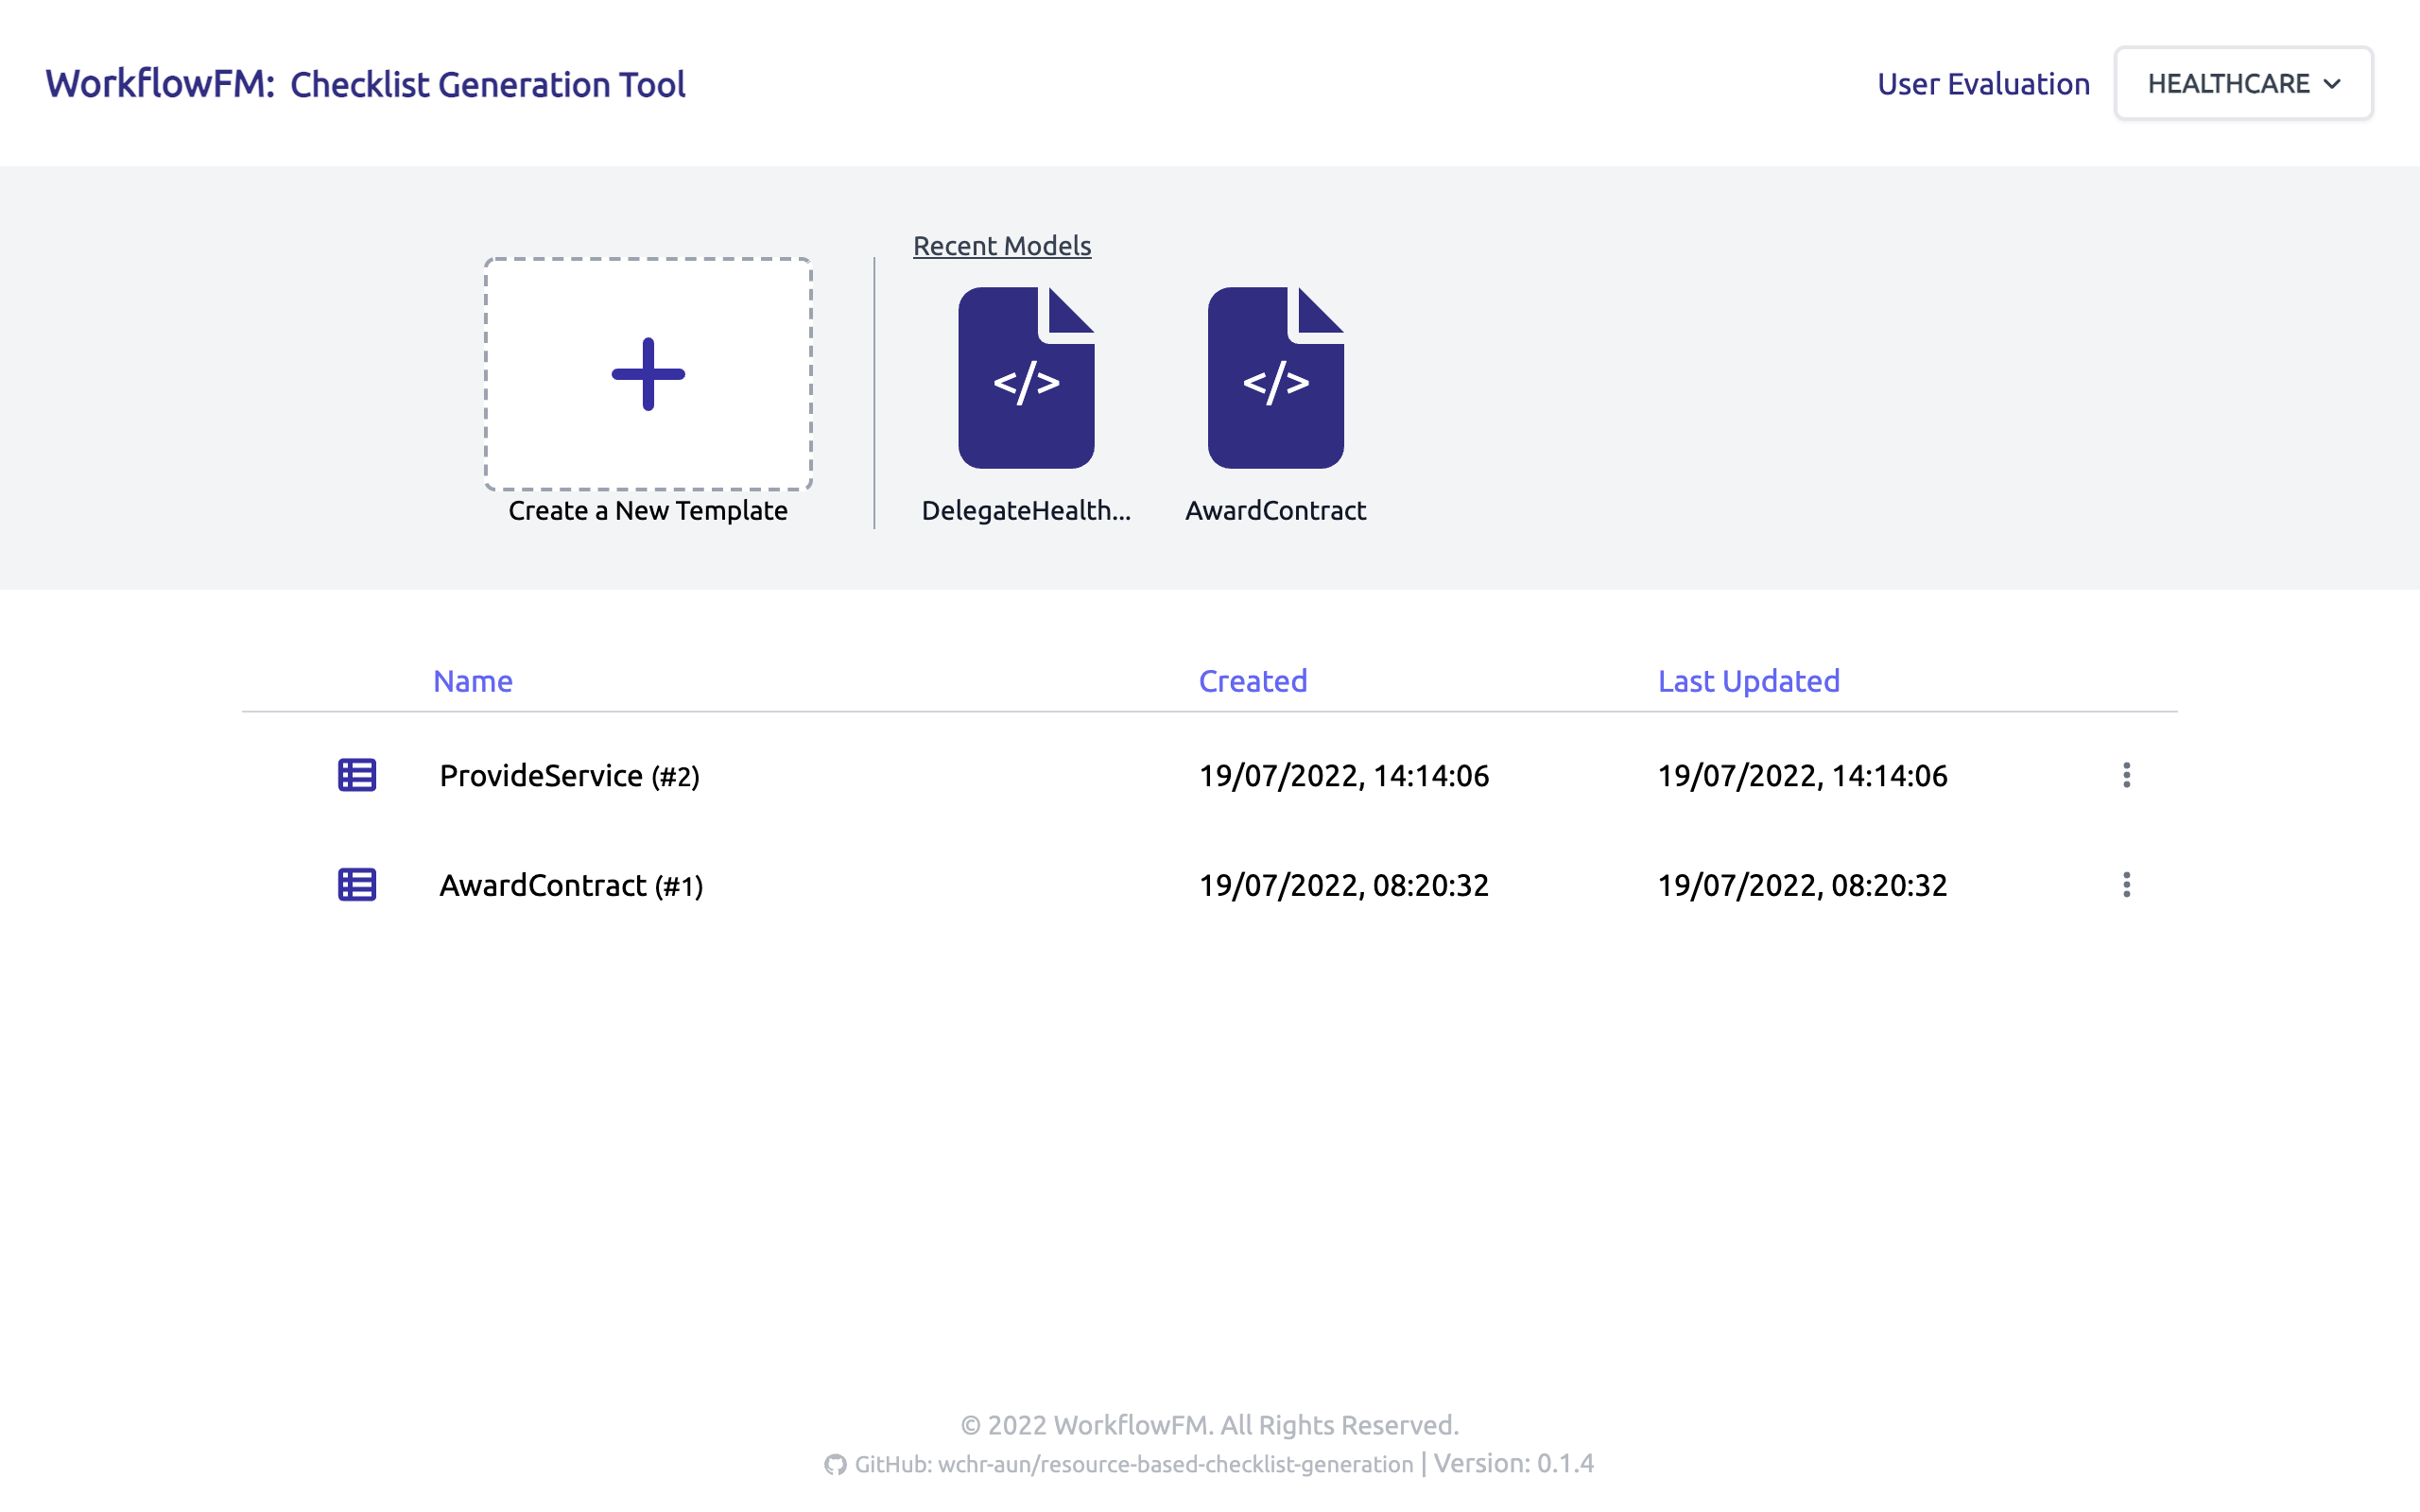
\includegraphics[width=0.6\textwidth]{overleaf/images/screens/main_screen.png}
    \caption{Main Screen}
    \label{fig:main_screen}
\end{figure}


\begin{figure}[ht!]
\centering
\begin{minipage}{.5\textwidth}
  \centering
  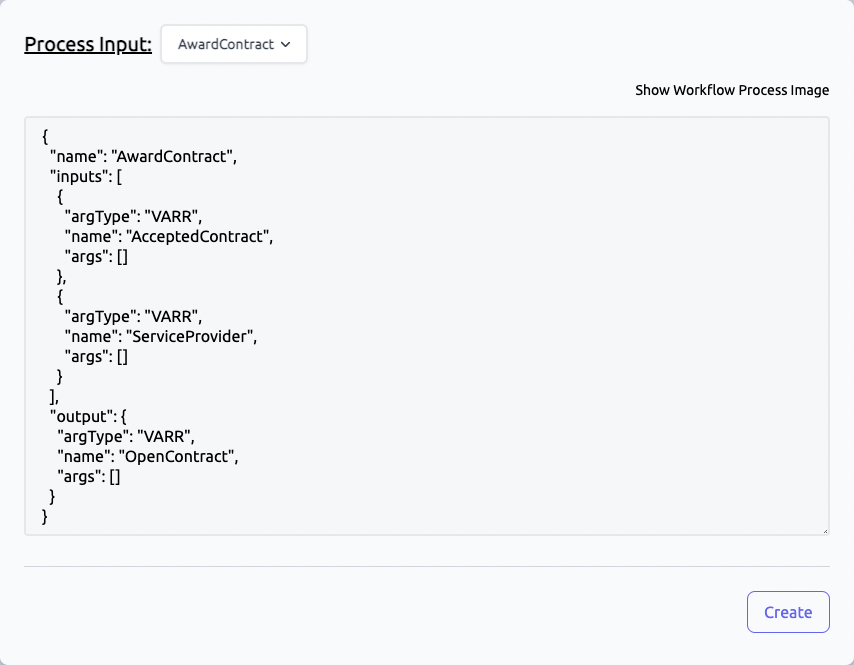
\includegraphics[width=0.9\linewidth]{overleaf/images/screens/process_input.png}
  \caption{Select Process Popup}
  \label{fig:process_input}
\end{minipage}%
\begin{minipage}{.5\textwidth}
  \centering
  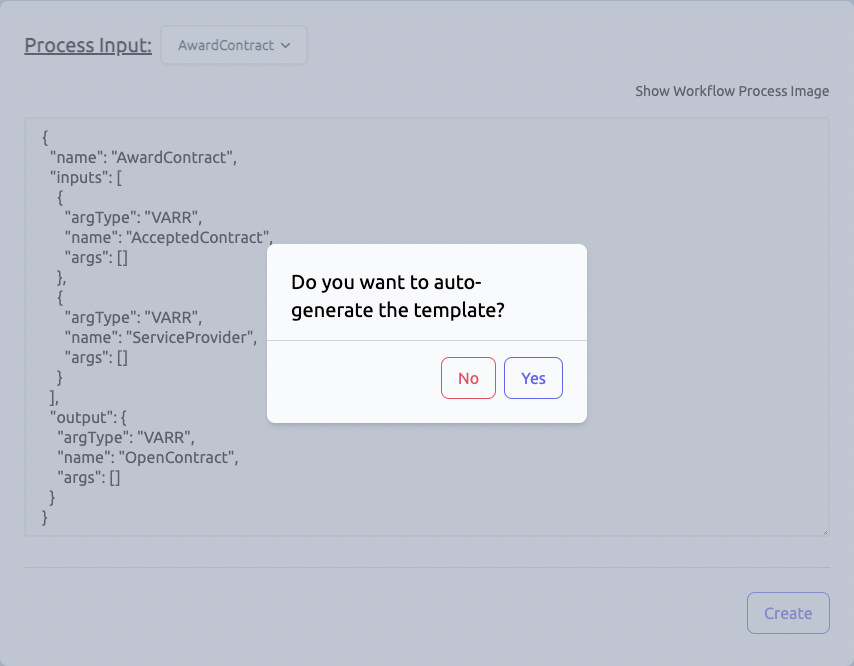
\includegraphics[width=0.9\linewidth]{overleaf/images/screens/autogen.png}
  \caption{Auto-Generation Popup}
  \label{fig:autogen}
\end{minipage}
\end{figure}




\subsection{Canvas}
\label{im:canvas}

In this section, we implemented three screens: Canvas Screen, Dependencies Management Popup, and Preview Screen. Similarly to Section \ref{im:landing}, we followed the navigation between these screens from Section \ref{interface_design} in the Design chapter.


% input information query here,
% query recommendation here,
% template saving here

\subsubsection{Canvas Screen}
\label{im:canvas_screen}

% This screen covers five functionalities, according to the software's structure section \ref{design:software_structure}: Template Creation, Input Information Query, Form Adjustment, Template Saving, and Query Recommendation.
% mention what this screen covers functionalities

As seen in Figure \ref{fig:canvas_screen}, the canvas screen contains three sections: checklist’s name, input information, and form adjustment. These sections are implemented following the checklist template's structure in Section \ref{checklist_strcuture}. The display name of each section can be edited. Other than the display names, the input information and the form adjustment sections can adjust the sequence order of what appears before or after as well as the visibility of each field, as shown in Figures \ref{fig:input_information_section} and \ref{fig:form_section}.

% \begin{figure}[ht!]
%     \centering
%     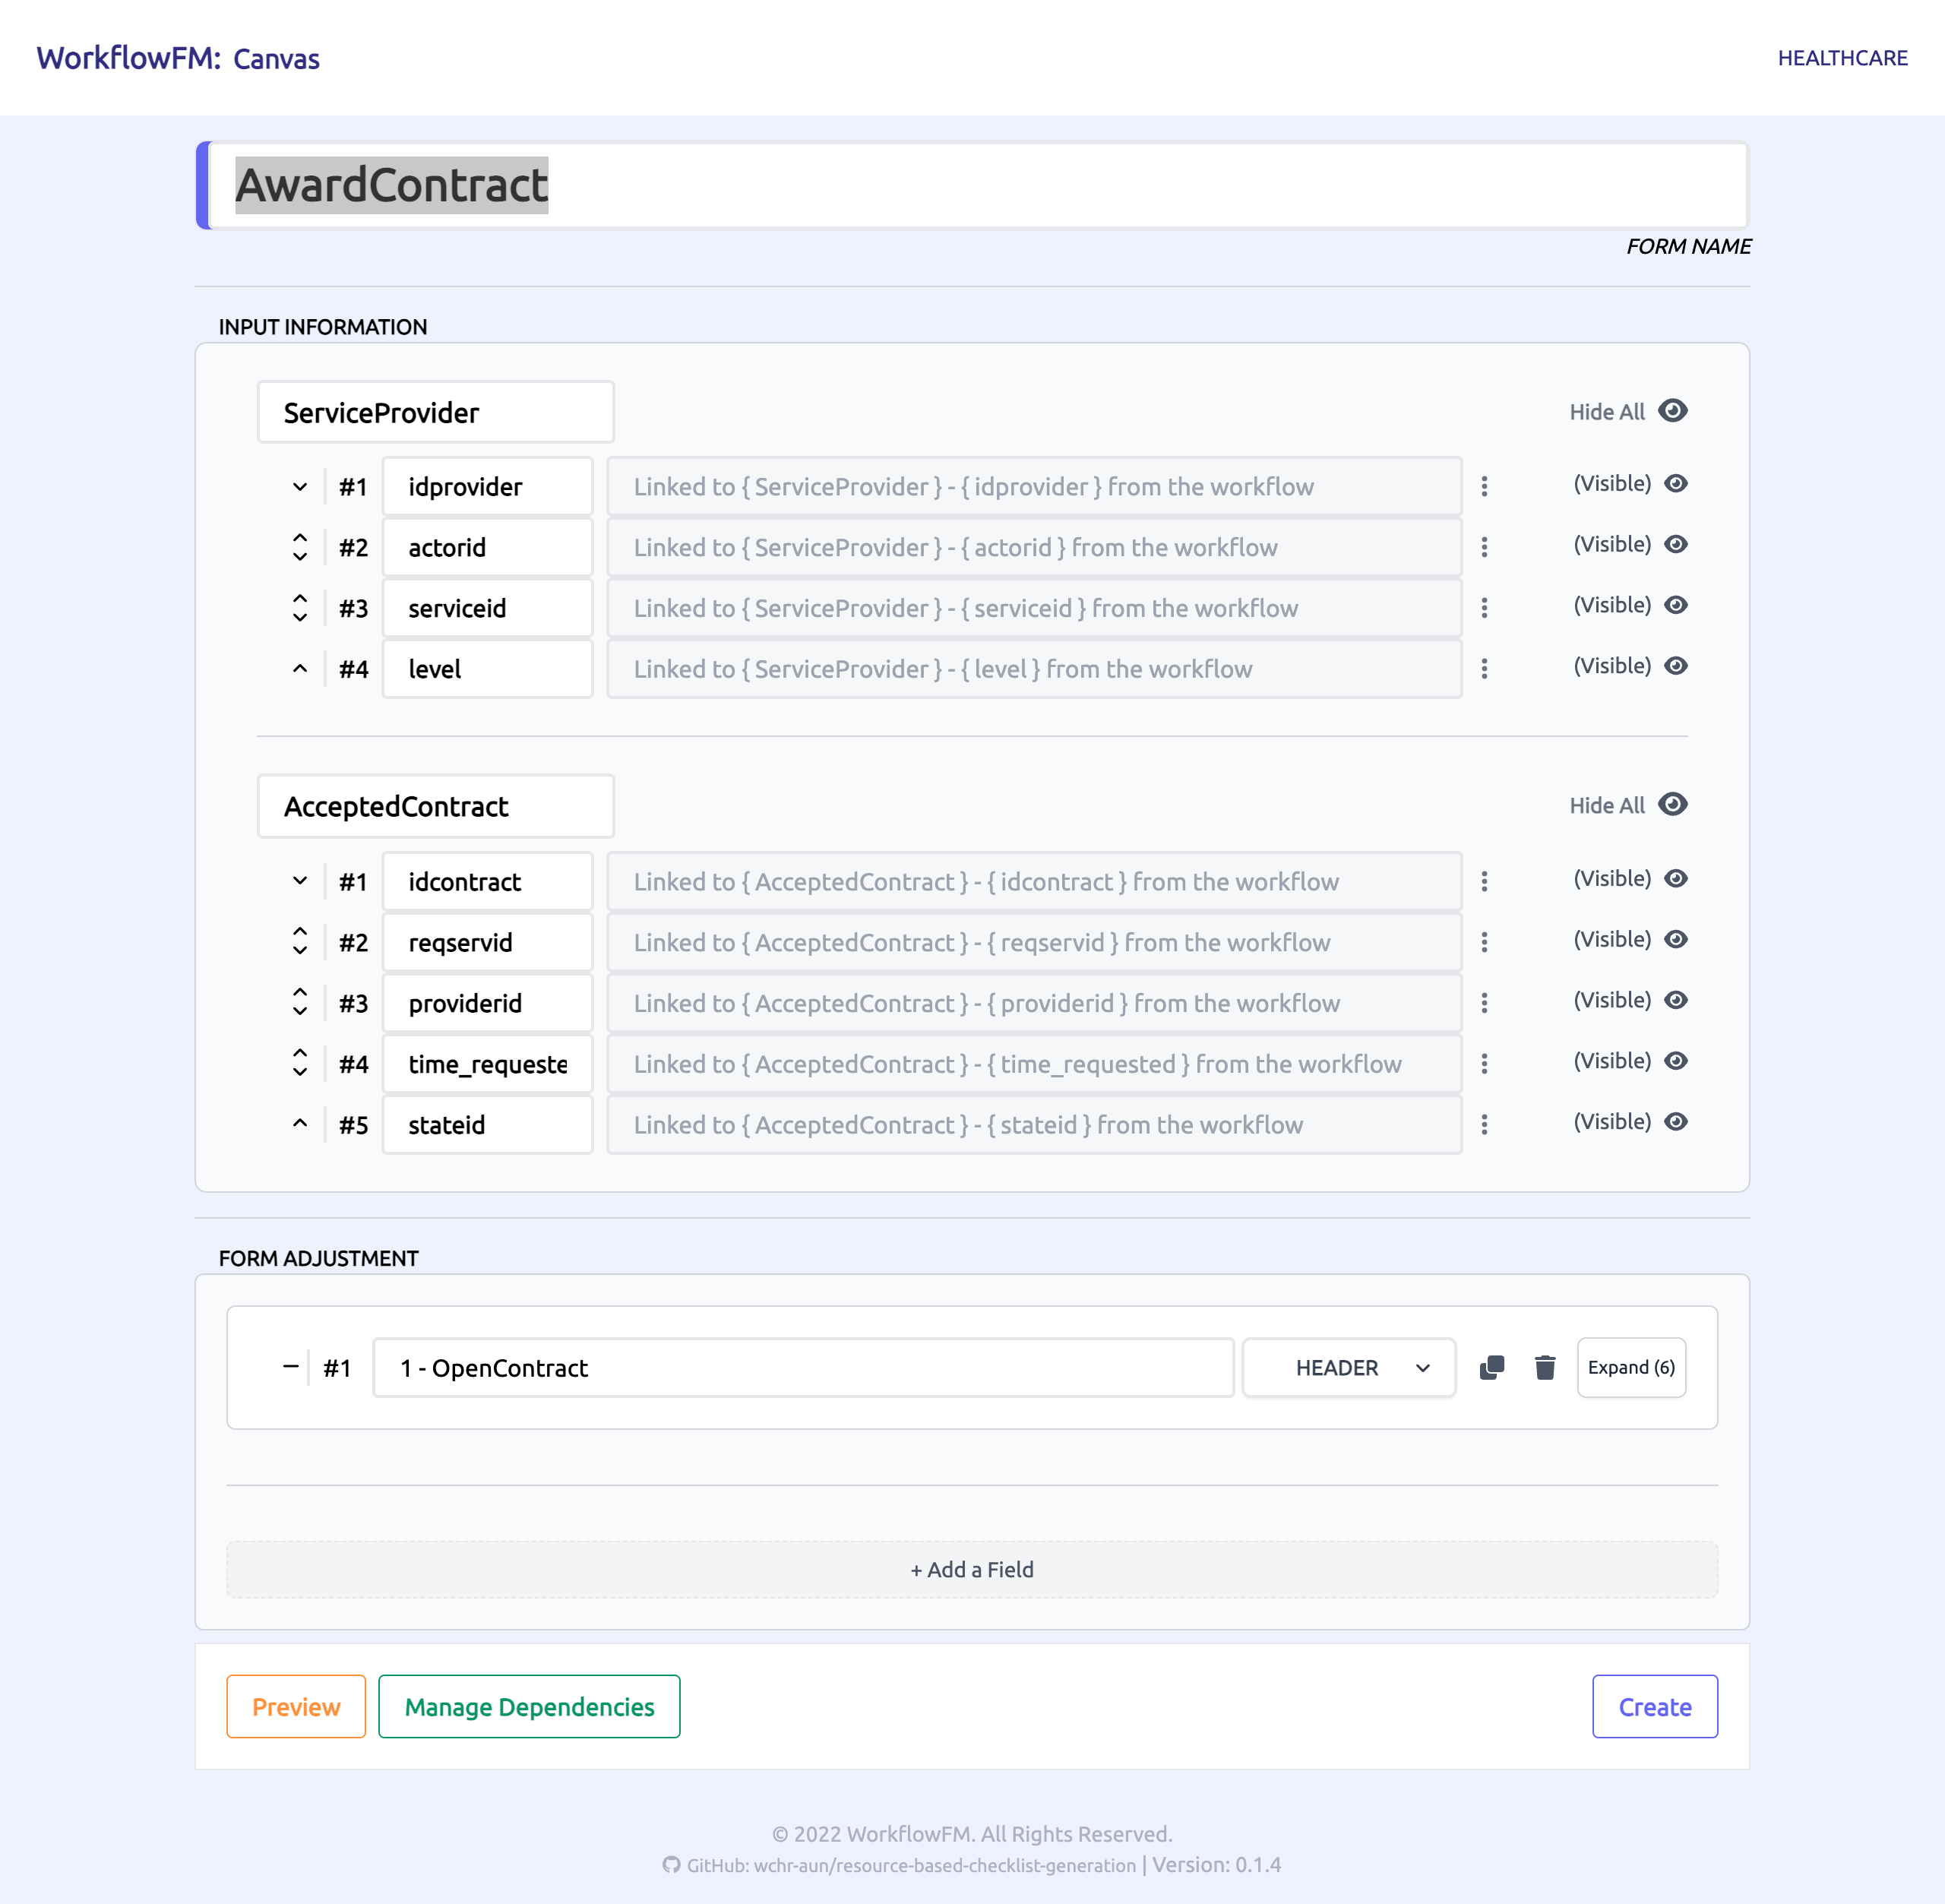
\includegraphics[width=0.6\textwidth]{overleaf/images/screens/canvas_screen.png}
%     \caption{Canvas Screen}
%     \label{fig:canvas_screen}
% \end{figure}

% form adjustment here
Designers can change the component type and the requirability of a component in the form adjustment section. There are ten component types: header, tab, textbox, paragraph, dropdown, choices, checkboxes, date, time, and constant. In addition, a new component can be added via the button at the bottom of each component. This all together is the \textbf{Form Adjustment} functionality.

\begin{figure}[ht!]
\centering
\begin{minipage}{.5\textwidth}
  \centering
  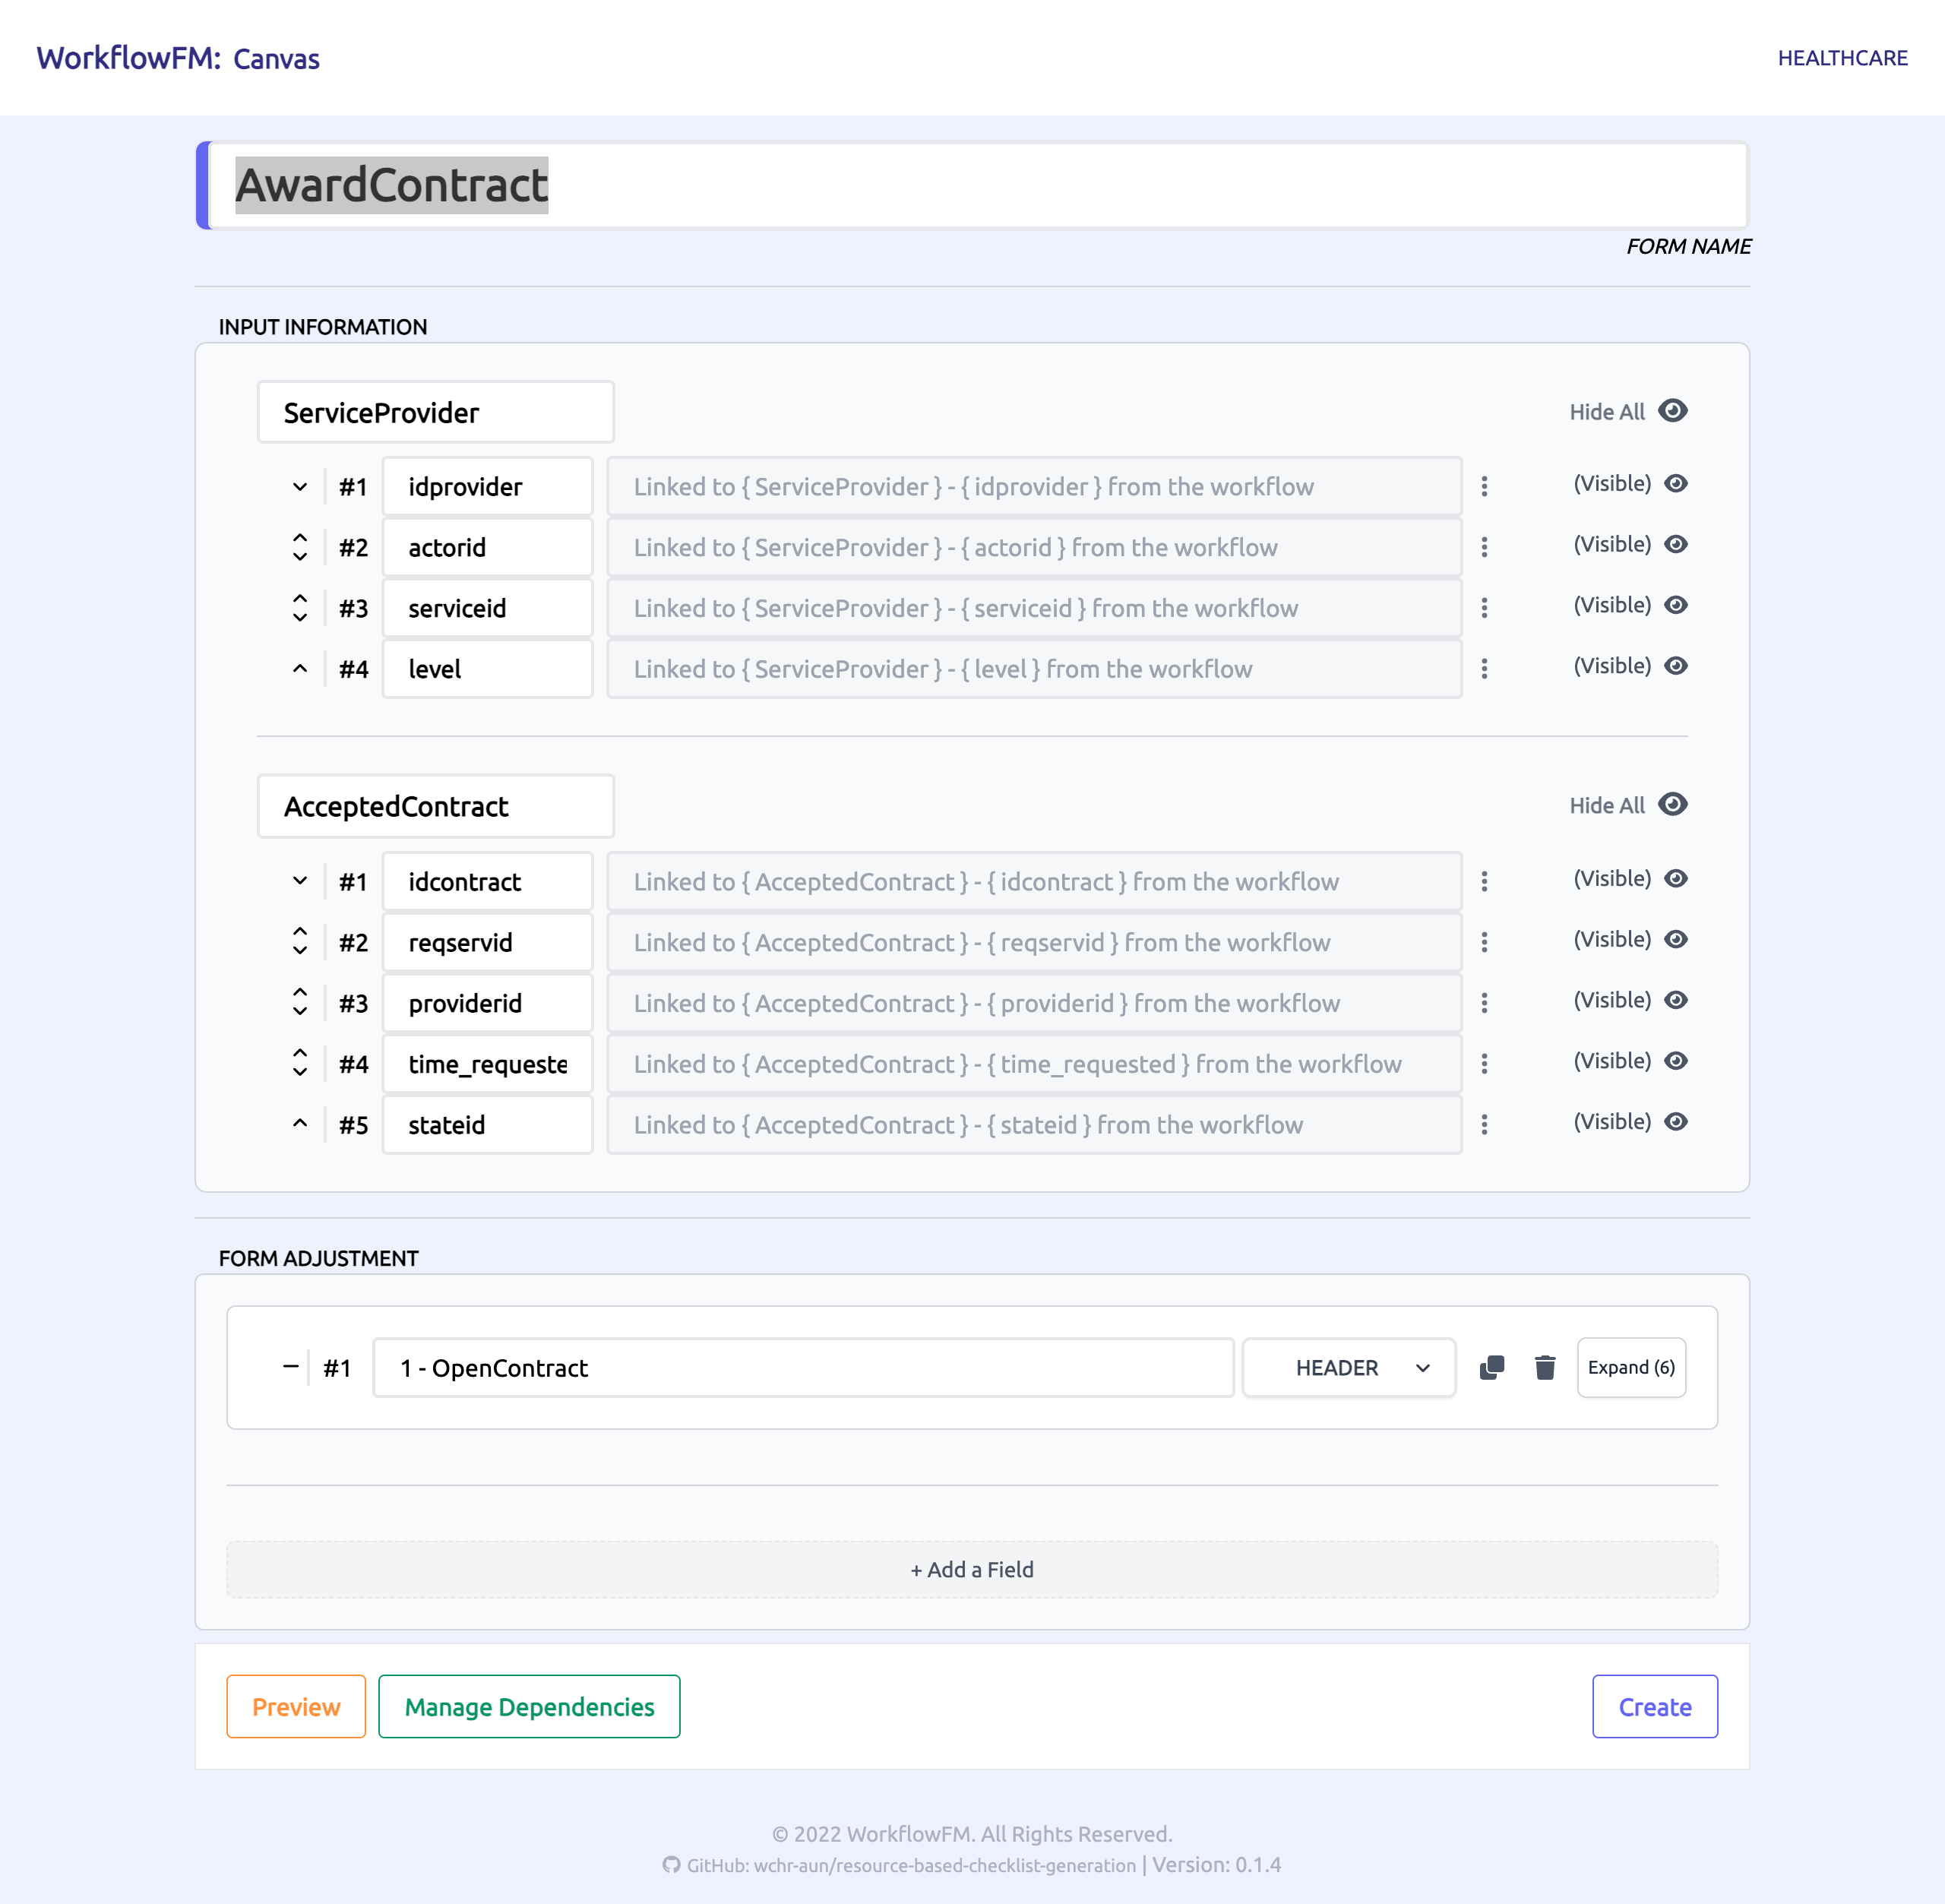
\includegraphics[width=0.9\linewidth]{overleaf/images/screens/canvas_screen.png}
  \caption{Canvas Screen}
  \label{fig:canvas_screen}
\end{minipage}%
\begin{minipage}{.5\textwidth}
  \centering
  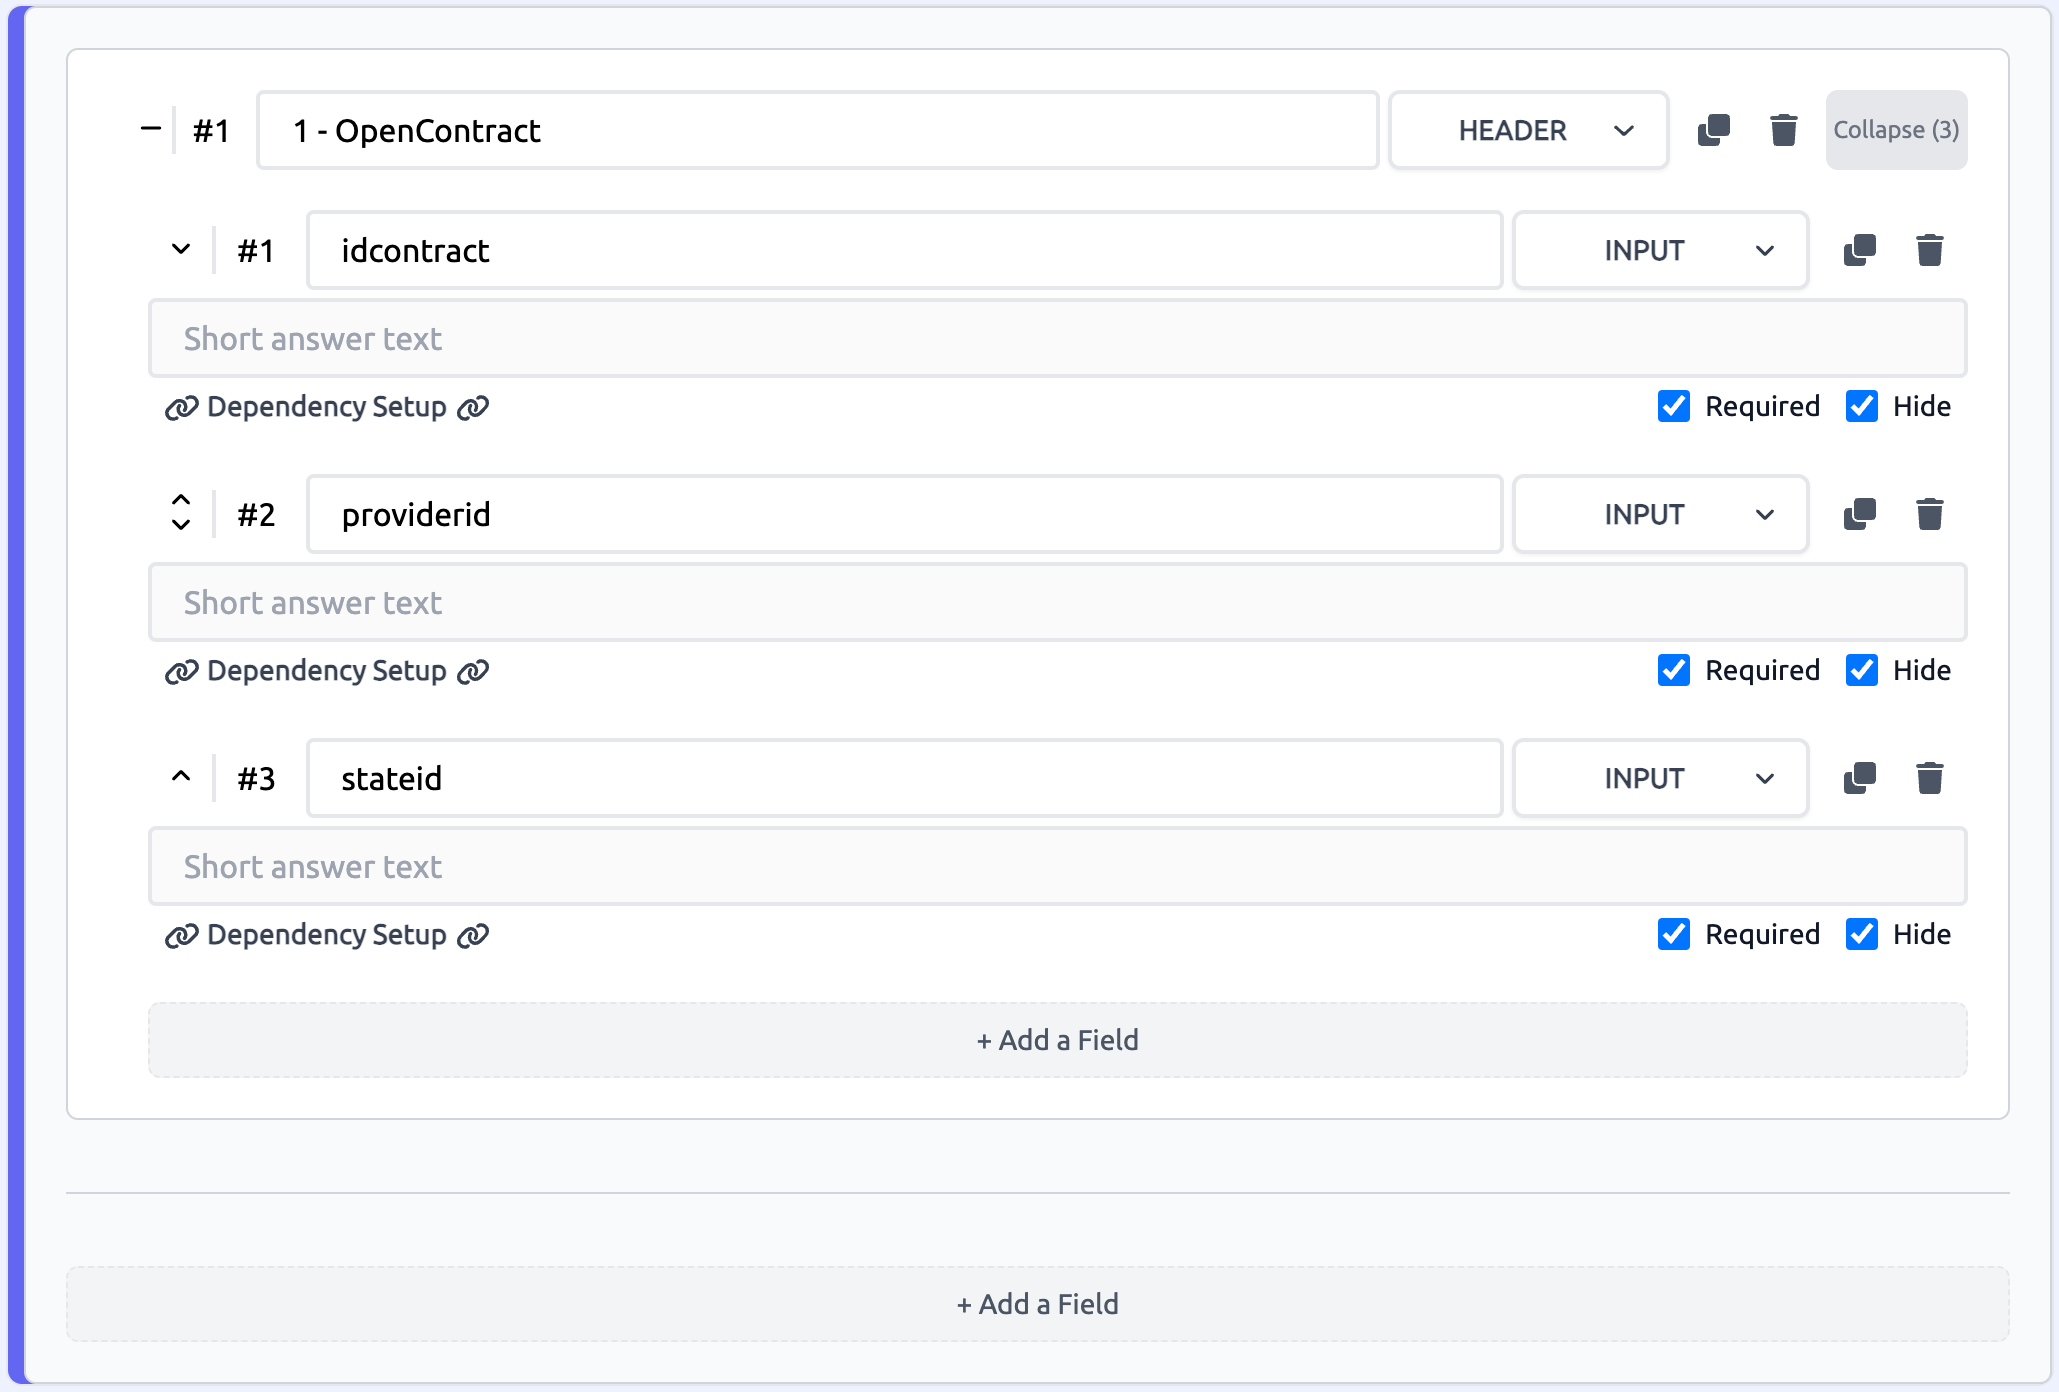
\includegraphics[width=0.9\linewidth]{overleaf/images/screens/form_section.png}
  \caption{Form Section}
  \label{fig:form_section}
\end{minipage}
\end{figure}


% Additional parts of the input infromation section
Additional to the input information section, new input information fields can be added through either ``Query more information using this field" or ``Get suggested query input information" options inside the vertical ellipsis icon (\vdots) in Figure \ref{fig:input_information_section}. This is the \textbf{Input Information Query} function. Selecting ``Get suggested query input information" will call the \textbf{Query Suggestion} function and display all the suggested fields, as shown in \ref{fig:query_suggestion}. Both the \textbf{Input Information Query} and the \textbf{Query Suggestion} functionalities will be further elaborated in Section \ref{backend_dependency}

There are two possible outcomes when selecting the ``Query more information using this field" option: i) a new field is added beneath the chosen field as seen in Figure \ref{fig:input_information_section}; and ii) a popup stating that this field has no relations displays. Designers can decide which field of an entity to display for the new input information field in the first scenario. It is important to note that the lists of entities and fields that are available depend on the field's relation. If the field contains no relation, the popup in the second scenario will appear. Upon selecting ``Get suggested query input information", if the field has at least one relation, the system will display a list of suggested input information fields to the designer, as shown in \ref{fig:query_suggestion}.

\begin{figure}[ht!]
\centering
\begin{minipage}{.5\textwidth}
  \centering
  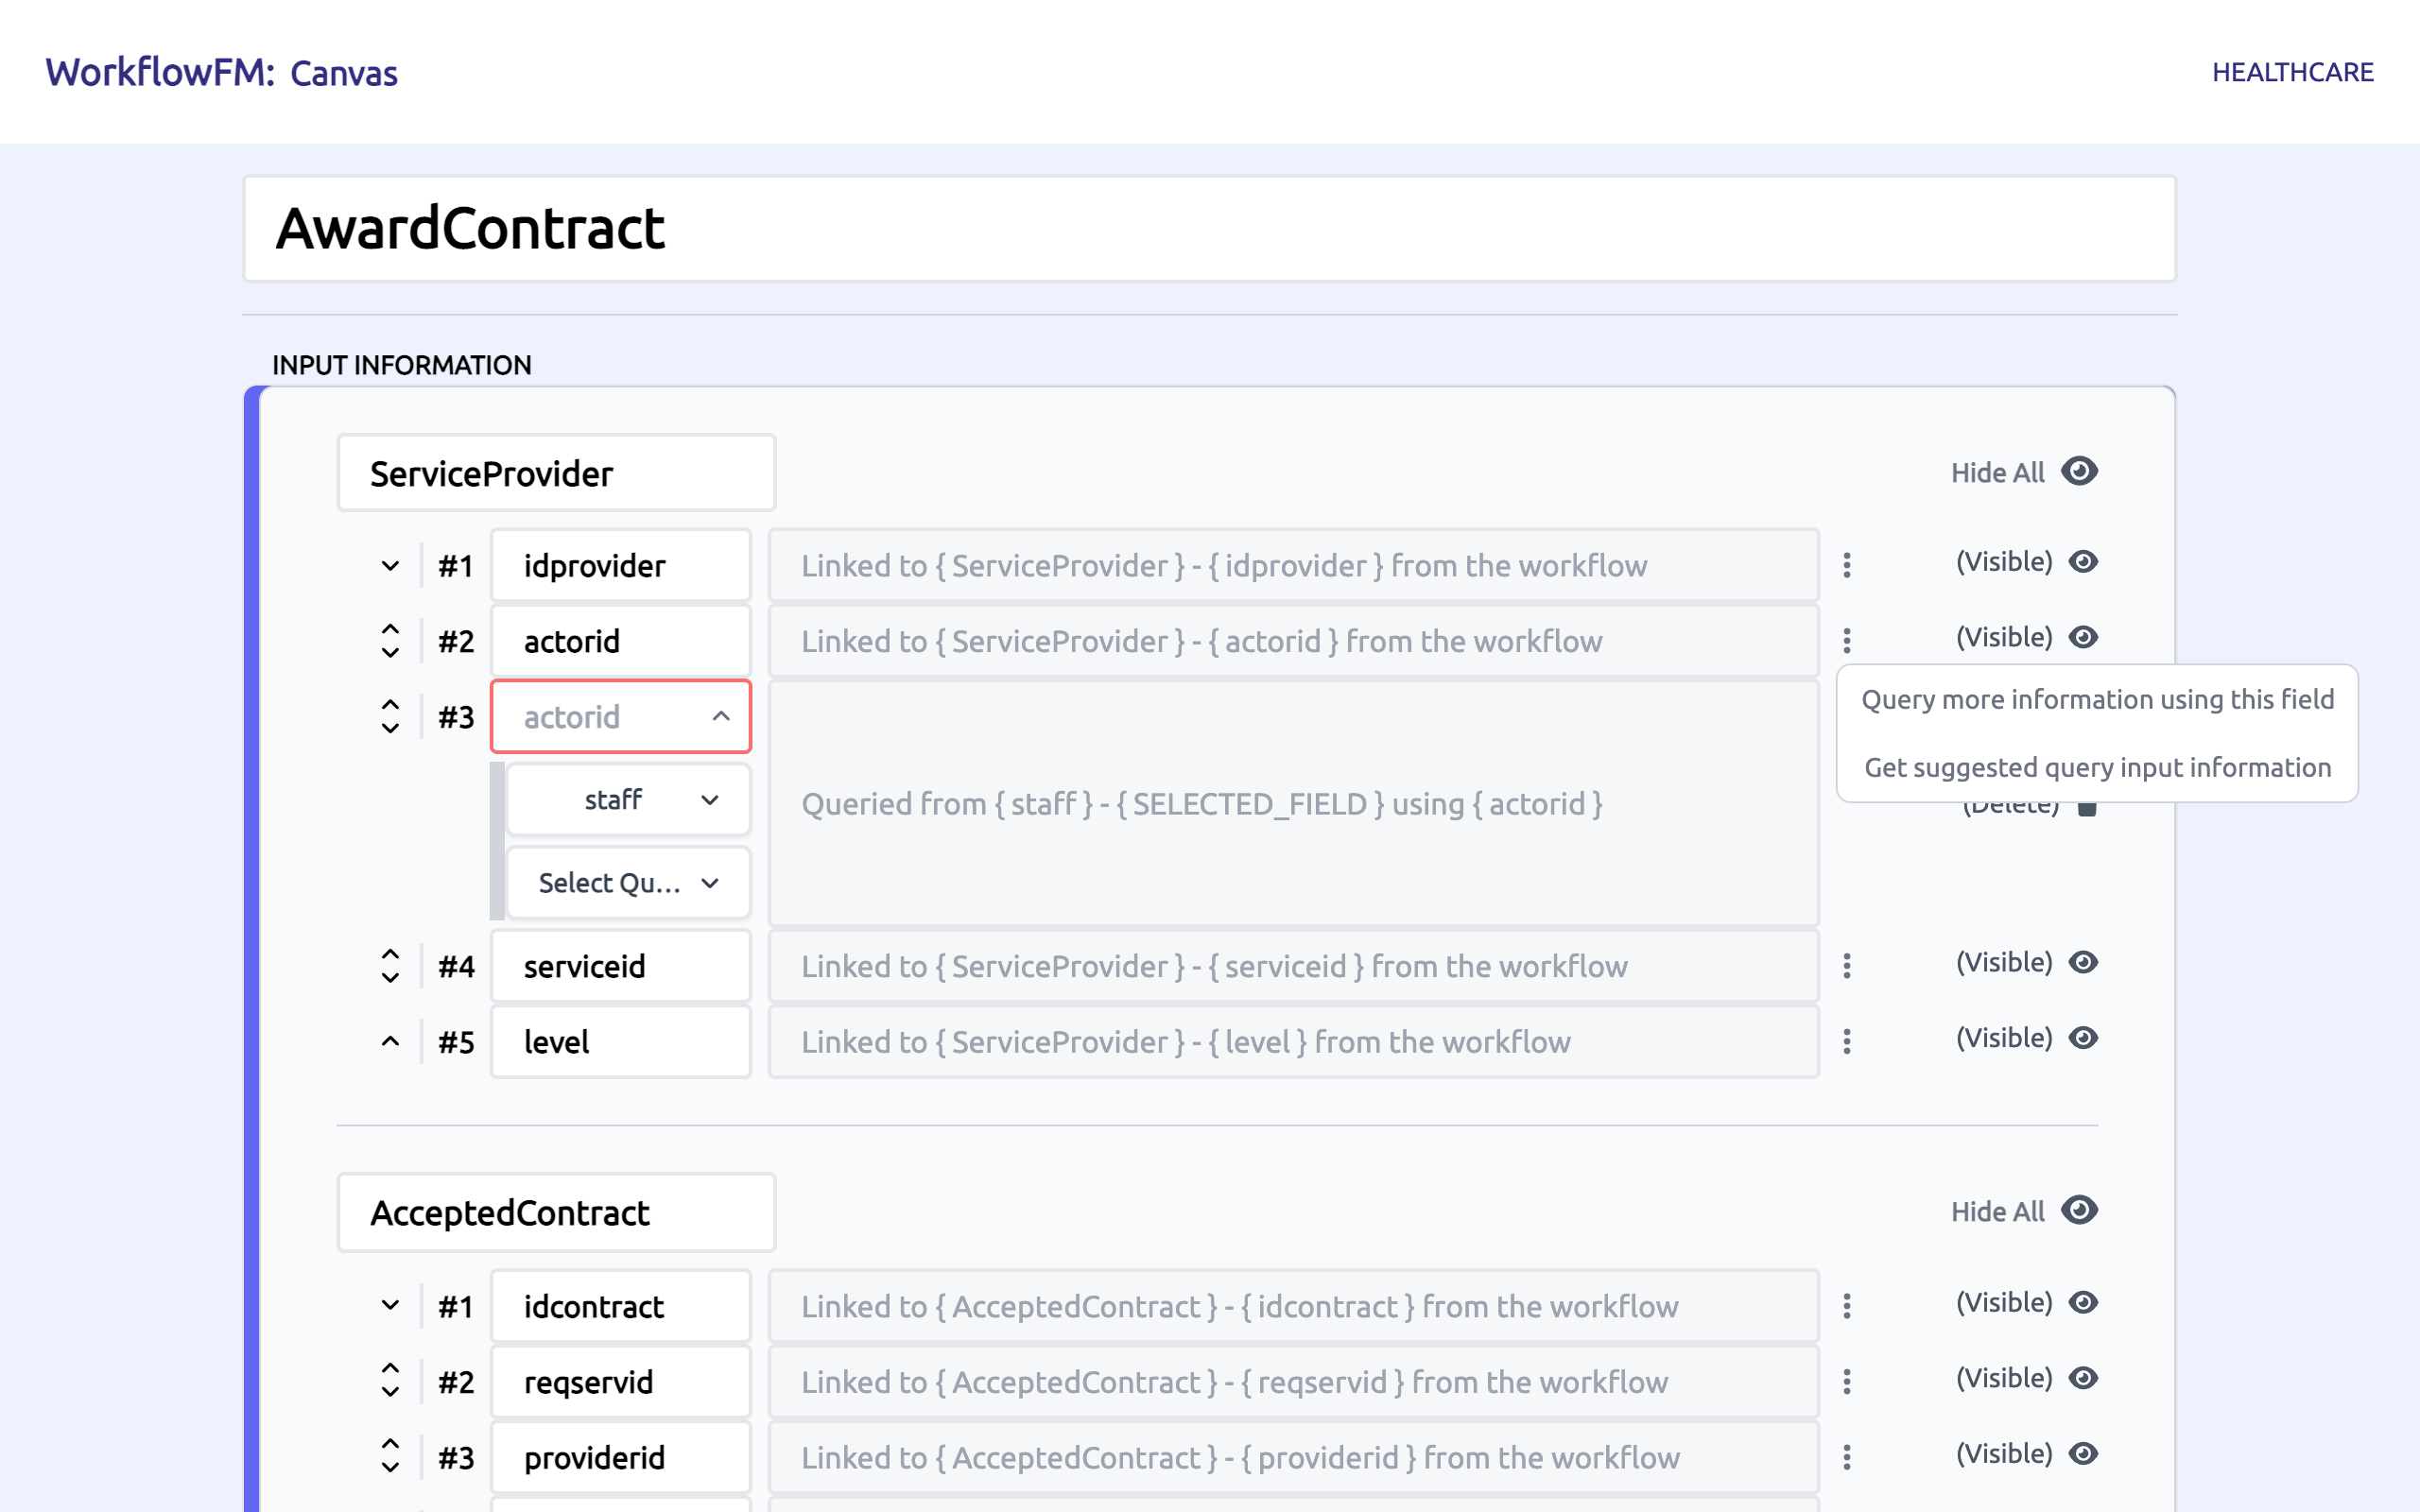
\includegraphics[width=0.9\linewidth]{overleaf/images/screens/input_information_section.png}
  \caption{Input Information Section}
  \label{fig:input_information_section}
\end{minipage}%
\begin{minipage}{.5\textwidth}
  \centering
  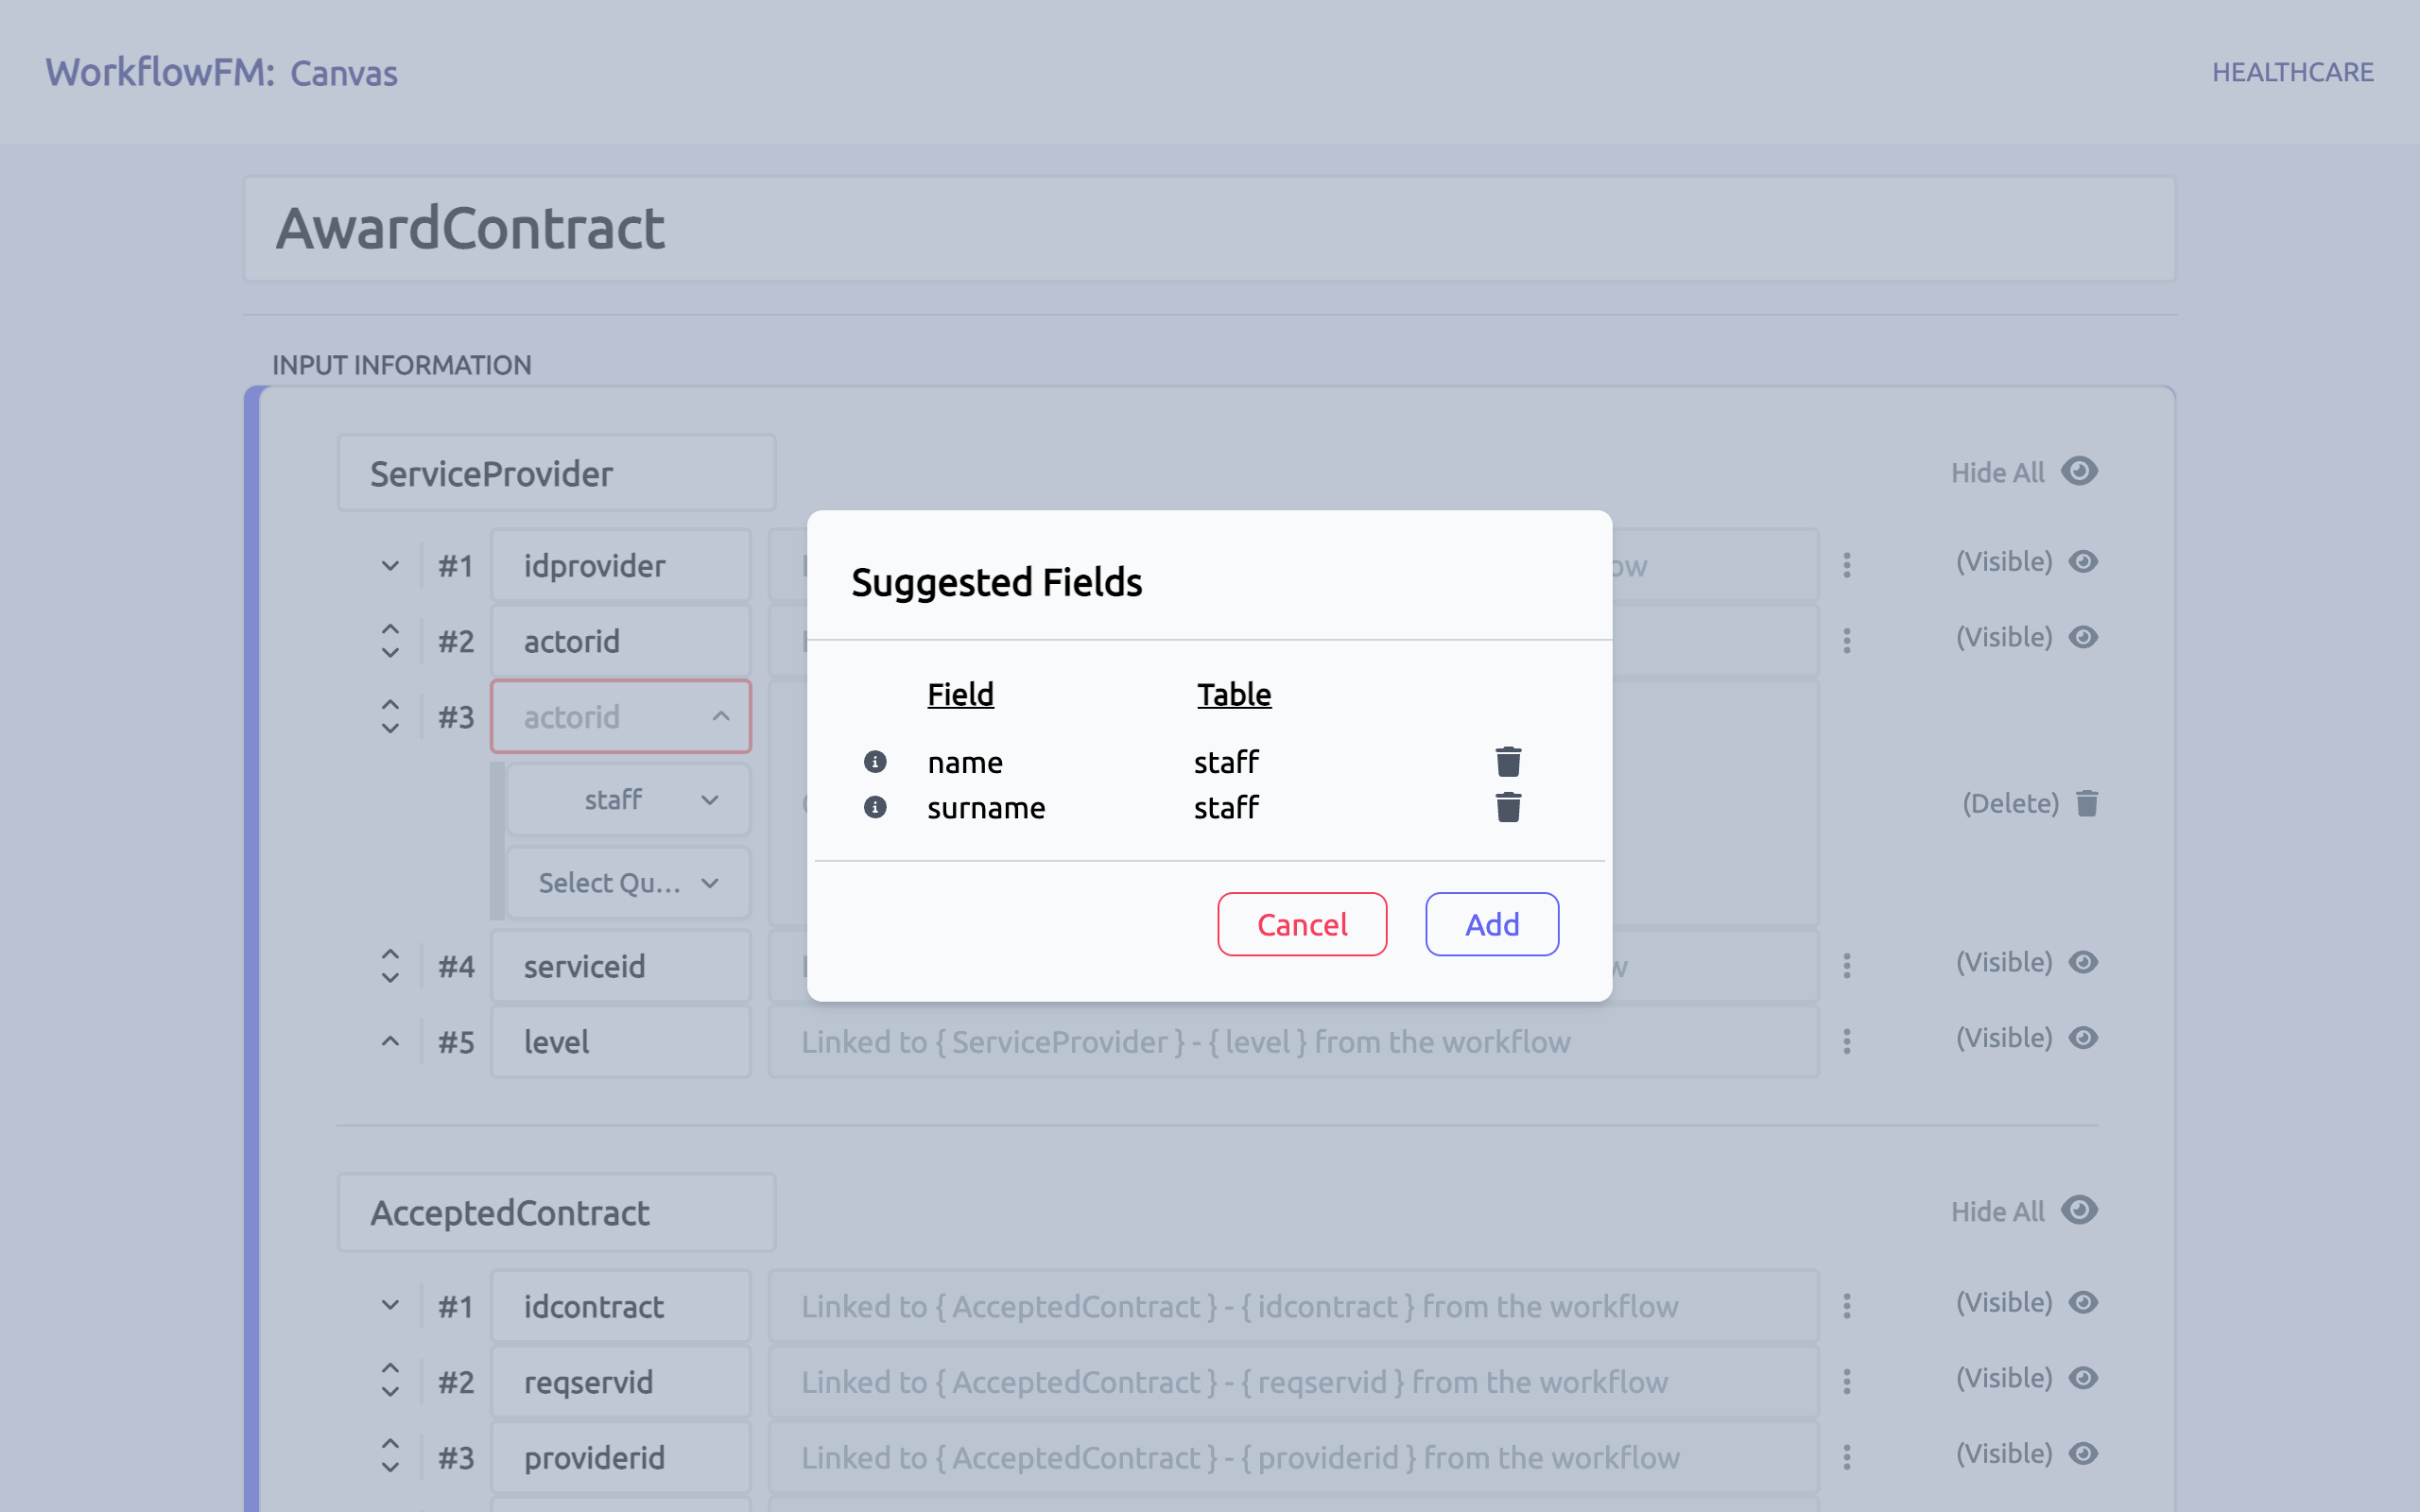
\includegraphics[width=0.9\linewidth]{overleaf/images/screens/query_suggestion.png}
  \caption{Query Suggestion Popup}
  \label{fig:query_suggestion}
\end{minipage}
\end{figure}


% \begin{figure}[ht!]
%     \centering
%     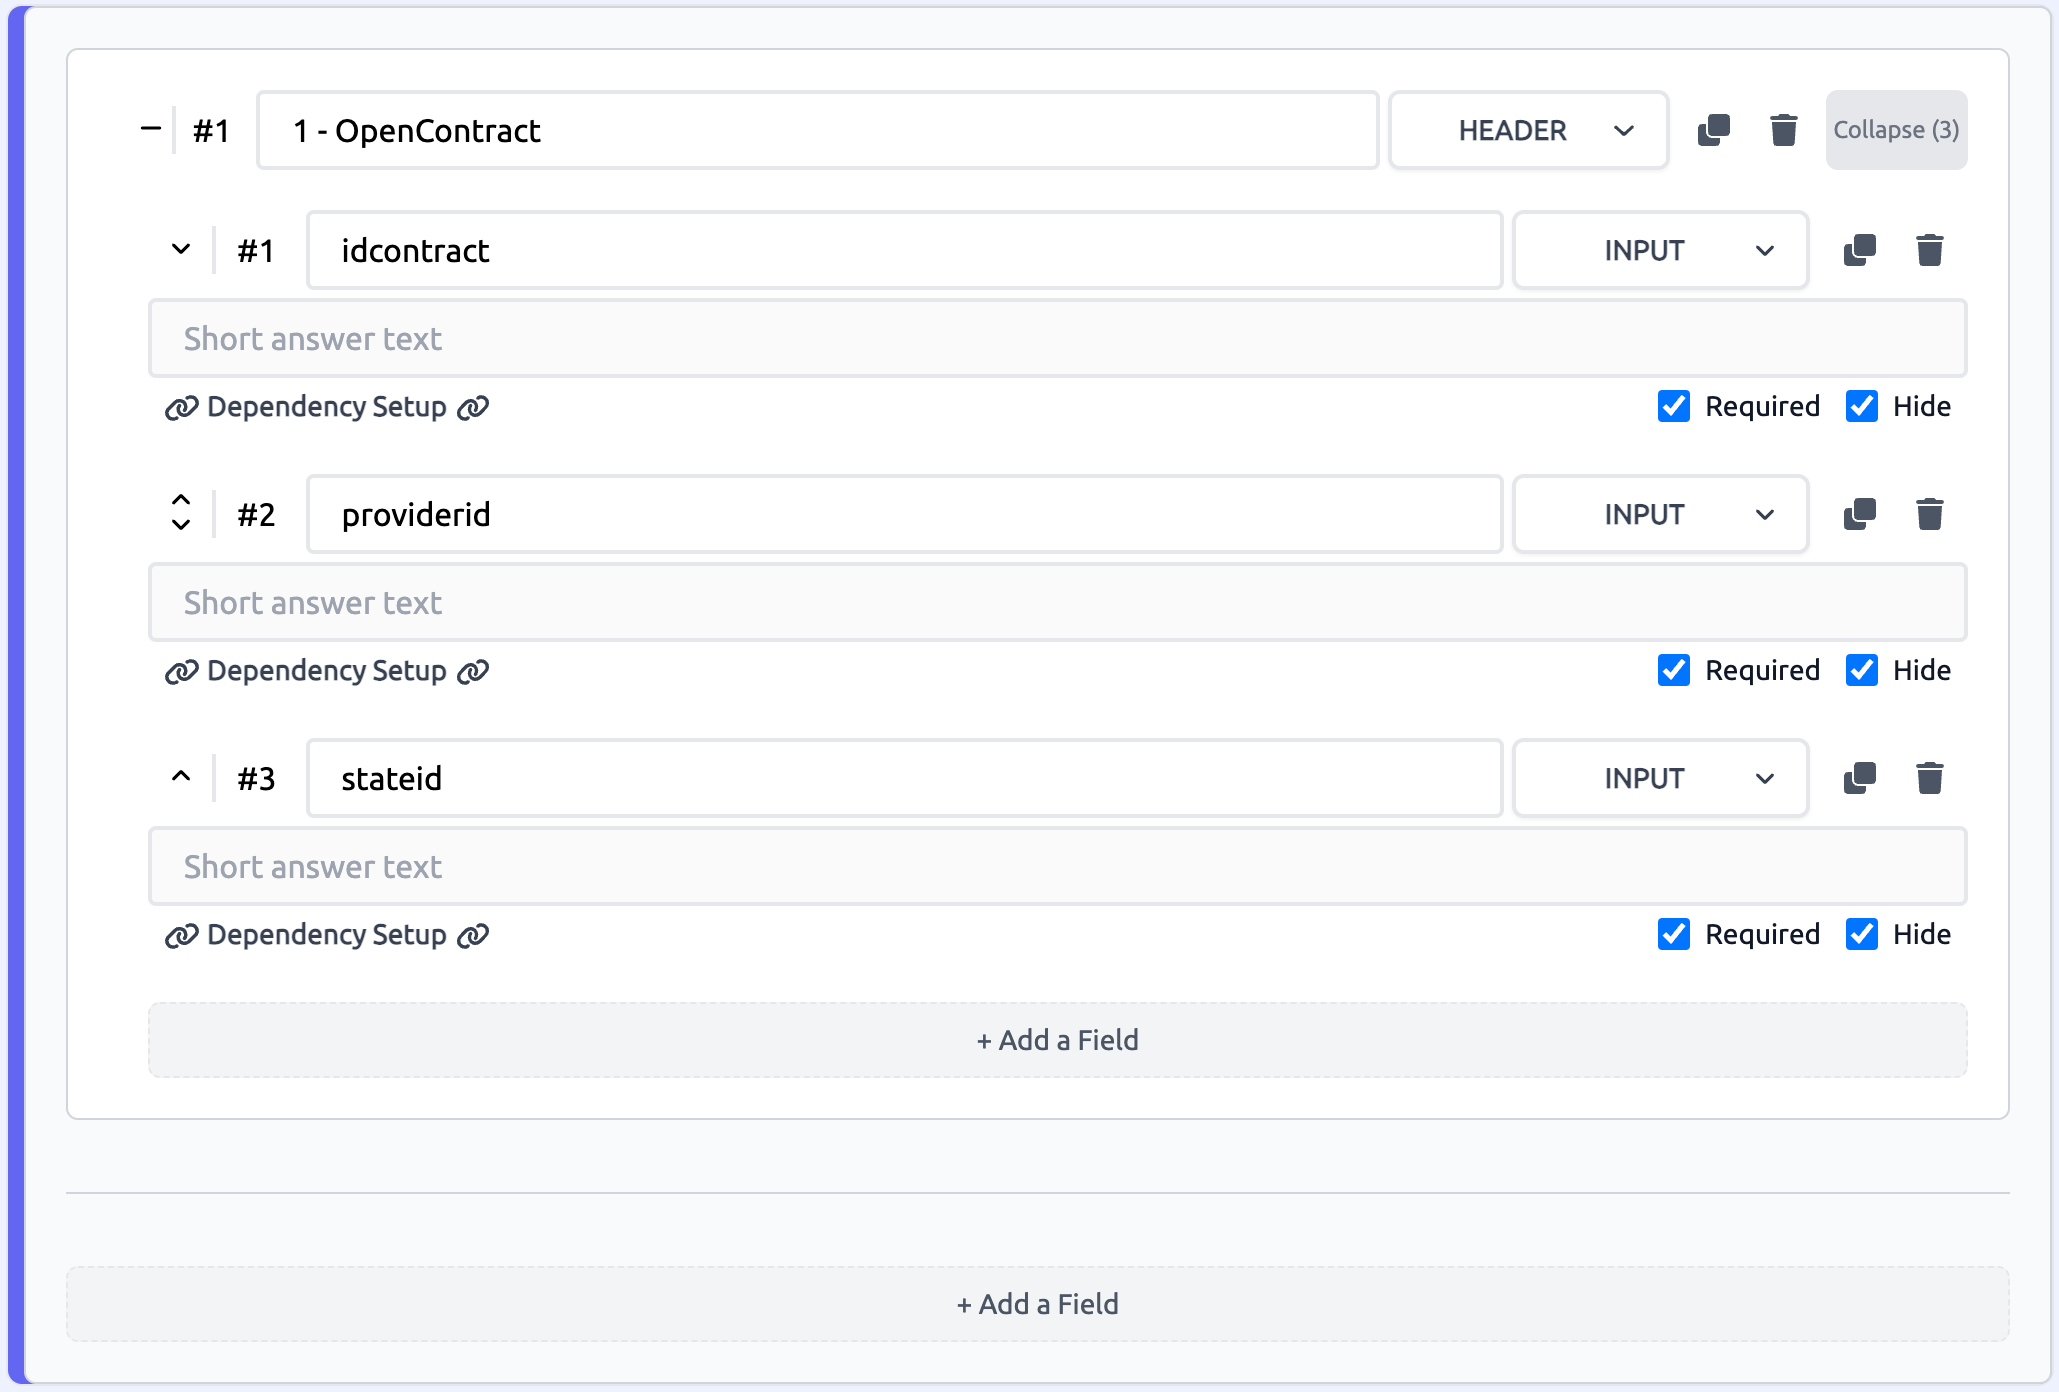
\includegraphics[width=0.5\textwidth]{overleaf/images/screens/form_section.png}
%     \caption{Form Section}
%     \label{fig:form_section}
% \end{figure}


\subsubsection{Dependencies Management Popups}
\label{im:depend_manage_pop}

Dependencies management popups can be accessed through the dependency setup button under each form component or the manage dependencies button at the bottom of the canvas screen (\ref{im:canvas_screen}). Accessing the dependency setup button will bring users to the component's dependencies setup. This popup is dedicated to each component, as shown in Figure \ref{fig:edit_dependencies_2}. On the other hand, the manage dependencies button will lead users to the all components' dependencies management popup, as seen in Figure \ref{fig:edit_dependencies}. Setting up input and output dependencies in these popups is part of the \textbf{Dependency Linking} function.


% DEPENDENCY VALIDATION DON'T FORGET IT!!!!
In the dependency management popup, users can validate dependencies by clicking the validate button. This is part of the \textbf{Dependencies Validation} functionality, which validates whether the output entities are all linked to a form component. For example, if the process's output contains an entity called ``Card Information", and the entity has three fields: card number, expired date, and security code. Each entity's field must be bound with a component in the form.

\begin{figure}[ht!]
\centering
\begin{minipage}{.5\textwidth}
  \centering
  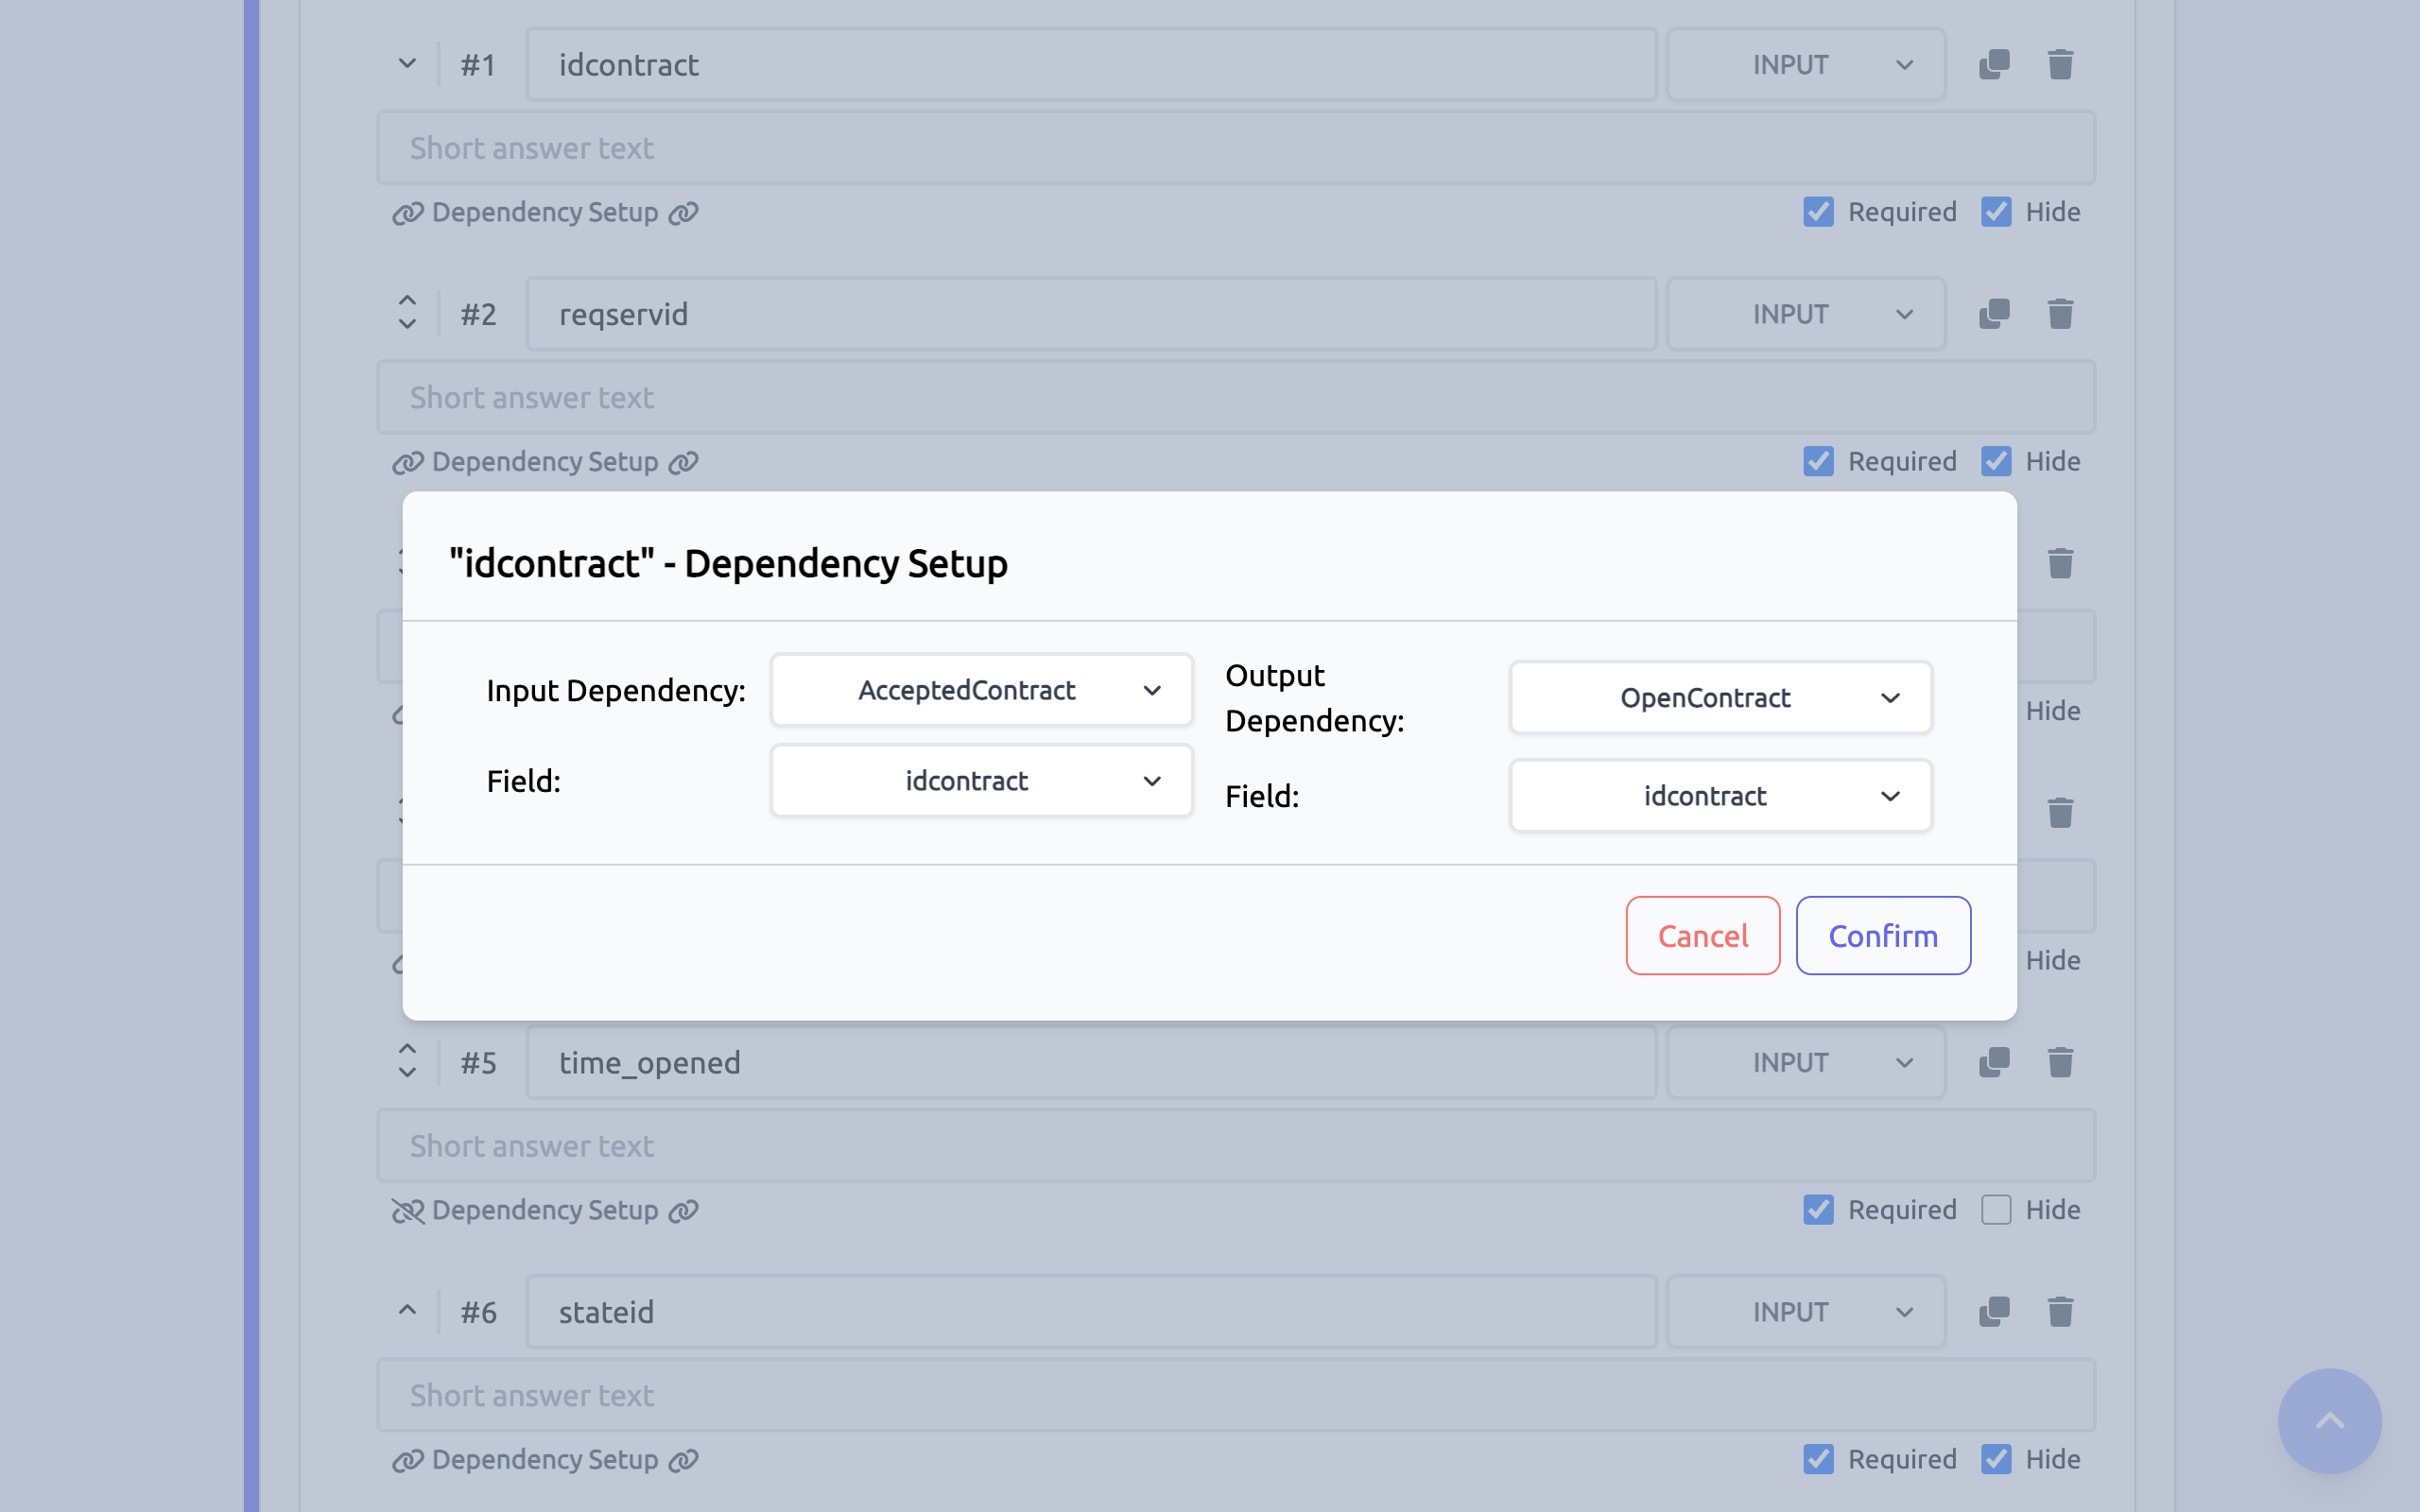
\includegraphics[width=0.9\linewidth]{overleaf/images/screens/edit_dependencies_2.png}
  \caption{Dependency Setup}
  \label{fig:edit_dependencies_2}
\end{minipage}%
\begin{minipage}{.5\textwidth}
  \centering
  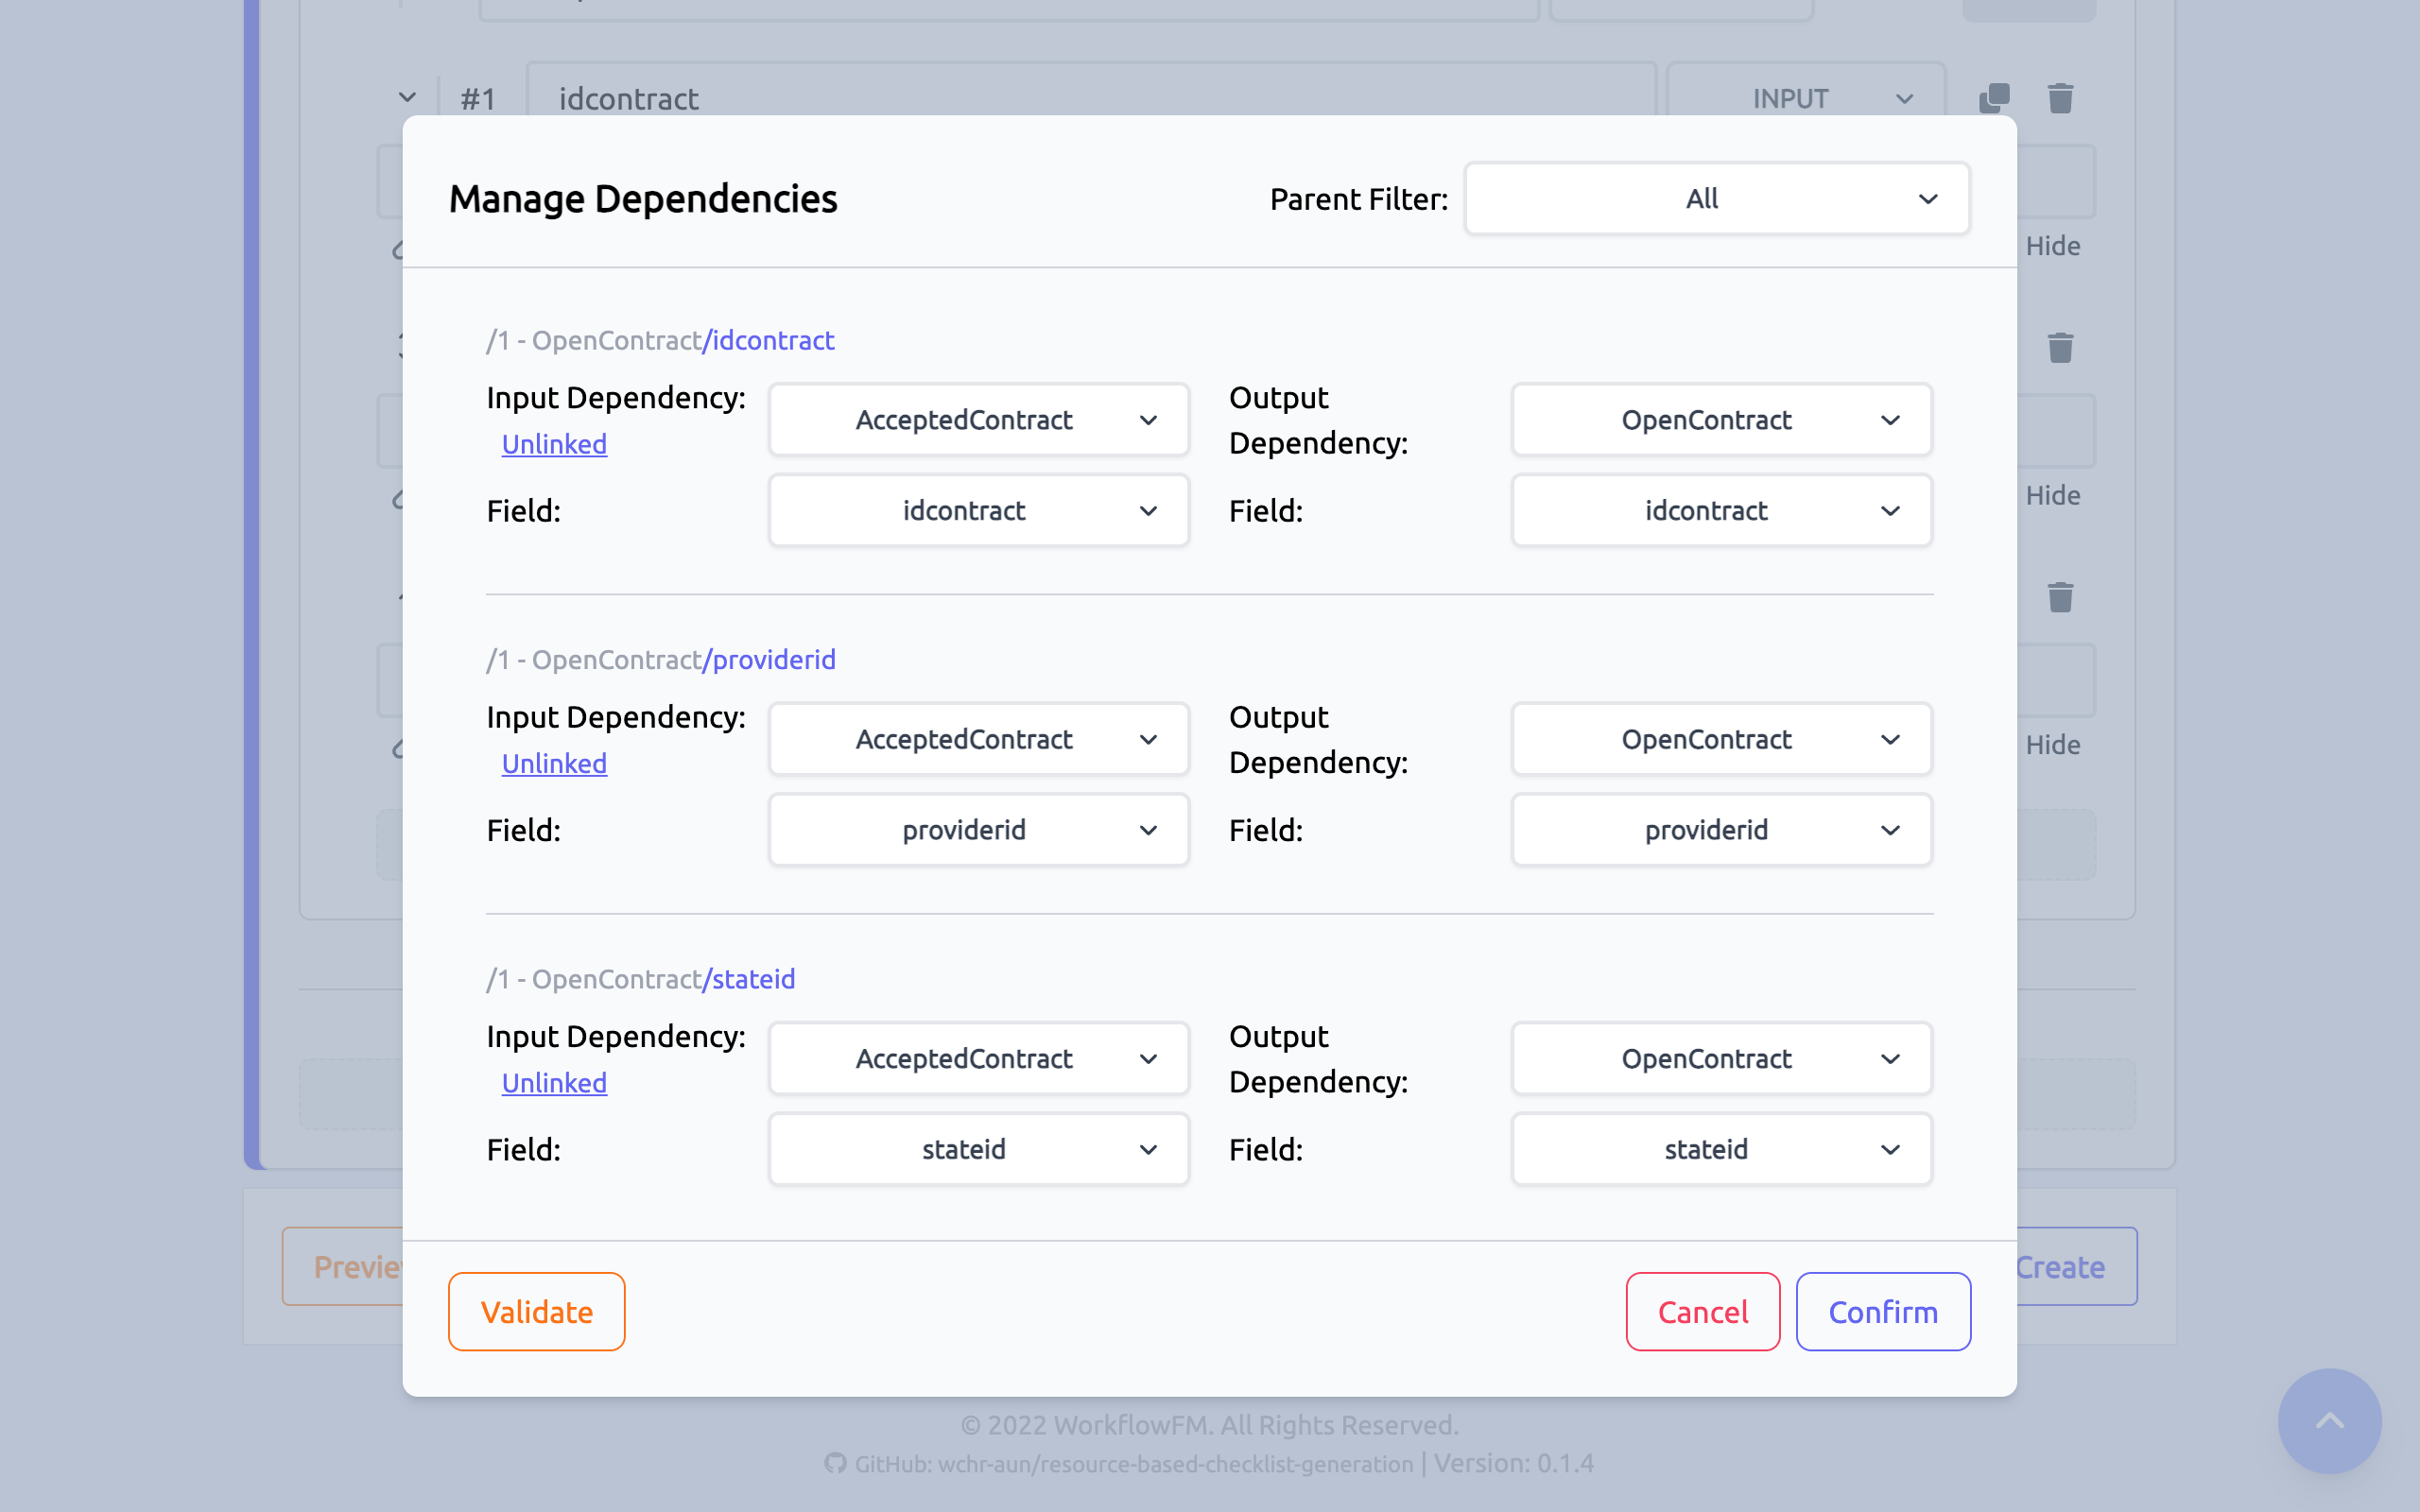
\includegraphics[width=0.9\linewidth]{overleaf/images/screens/edit_dependencies.png}
  \caption{Dependencies Management}
  \label{fig:edit_dependencies}
\end{minipage}
\end{figure}

\subsubsection{Preview Screen}
\label{im:preview_screen}

Preview screen is the screen that allows users to visualise how the template would look like when it is created, which is illustrated in Figure \ref{fig:preview_screen}. This screen can be accessed through the preview button in the canvas screen (\ref{im:canvas_screen}). Additionally, this screen shares the same interface with the checklist screen (\ref{im:view_checklist}).



\begin{figure}[ht!]
\centering
\begin{minipage}{.5\textwidth}
  \centering
    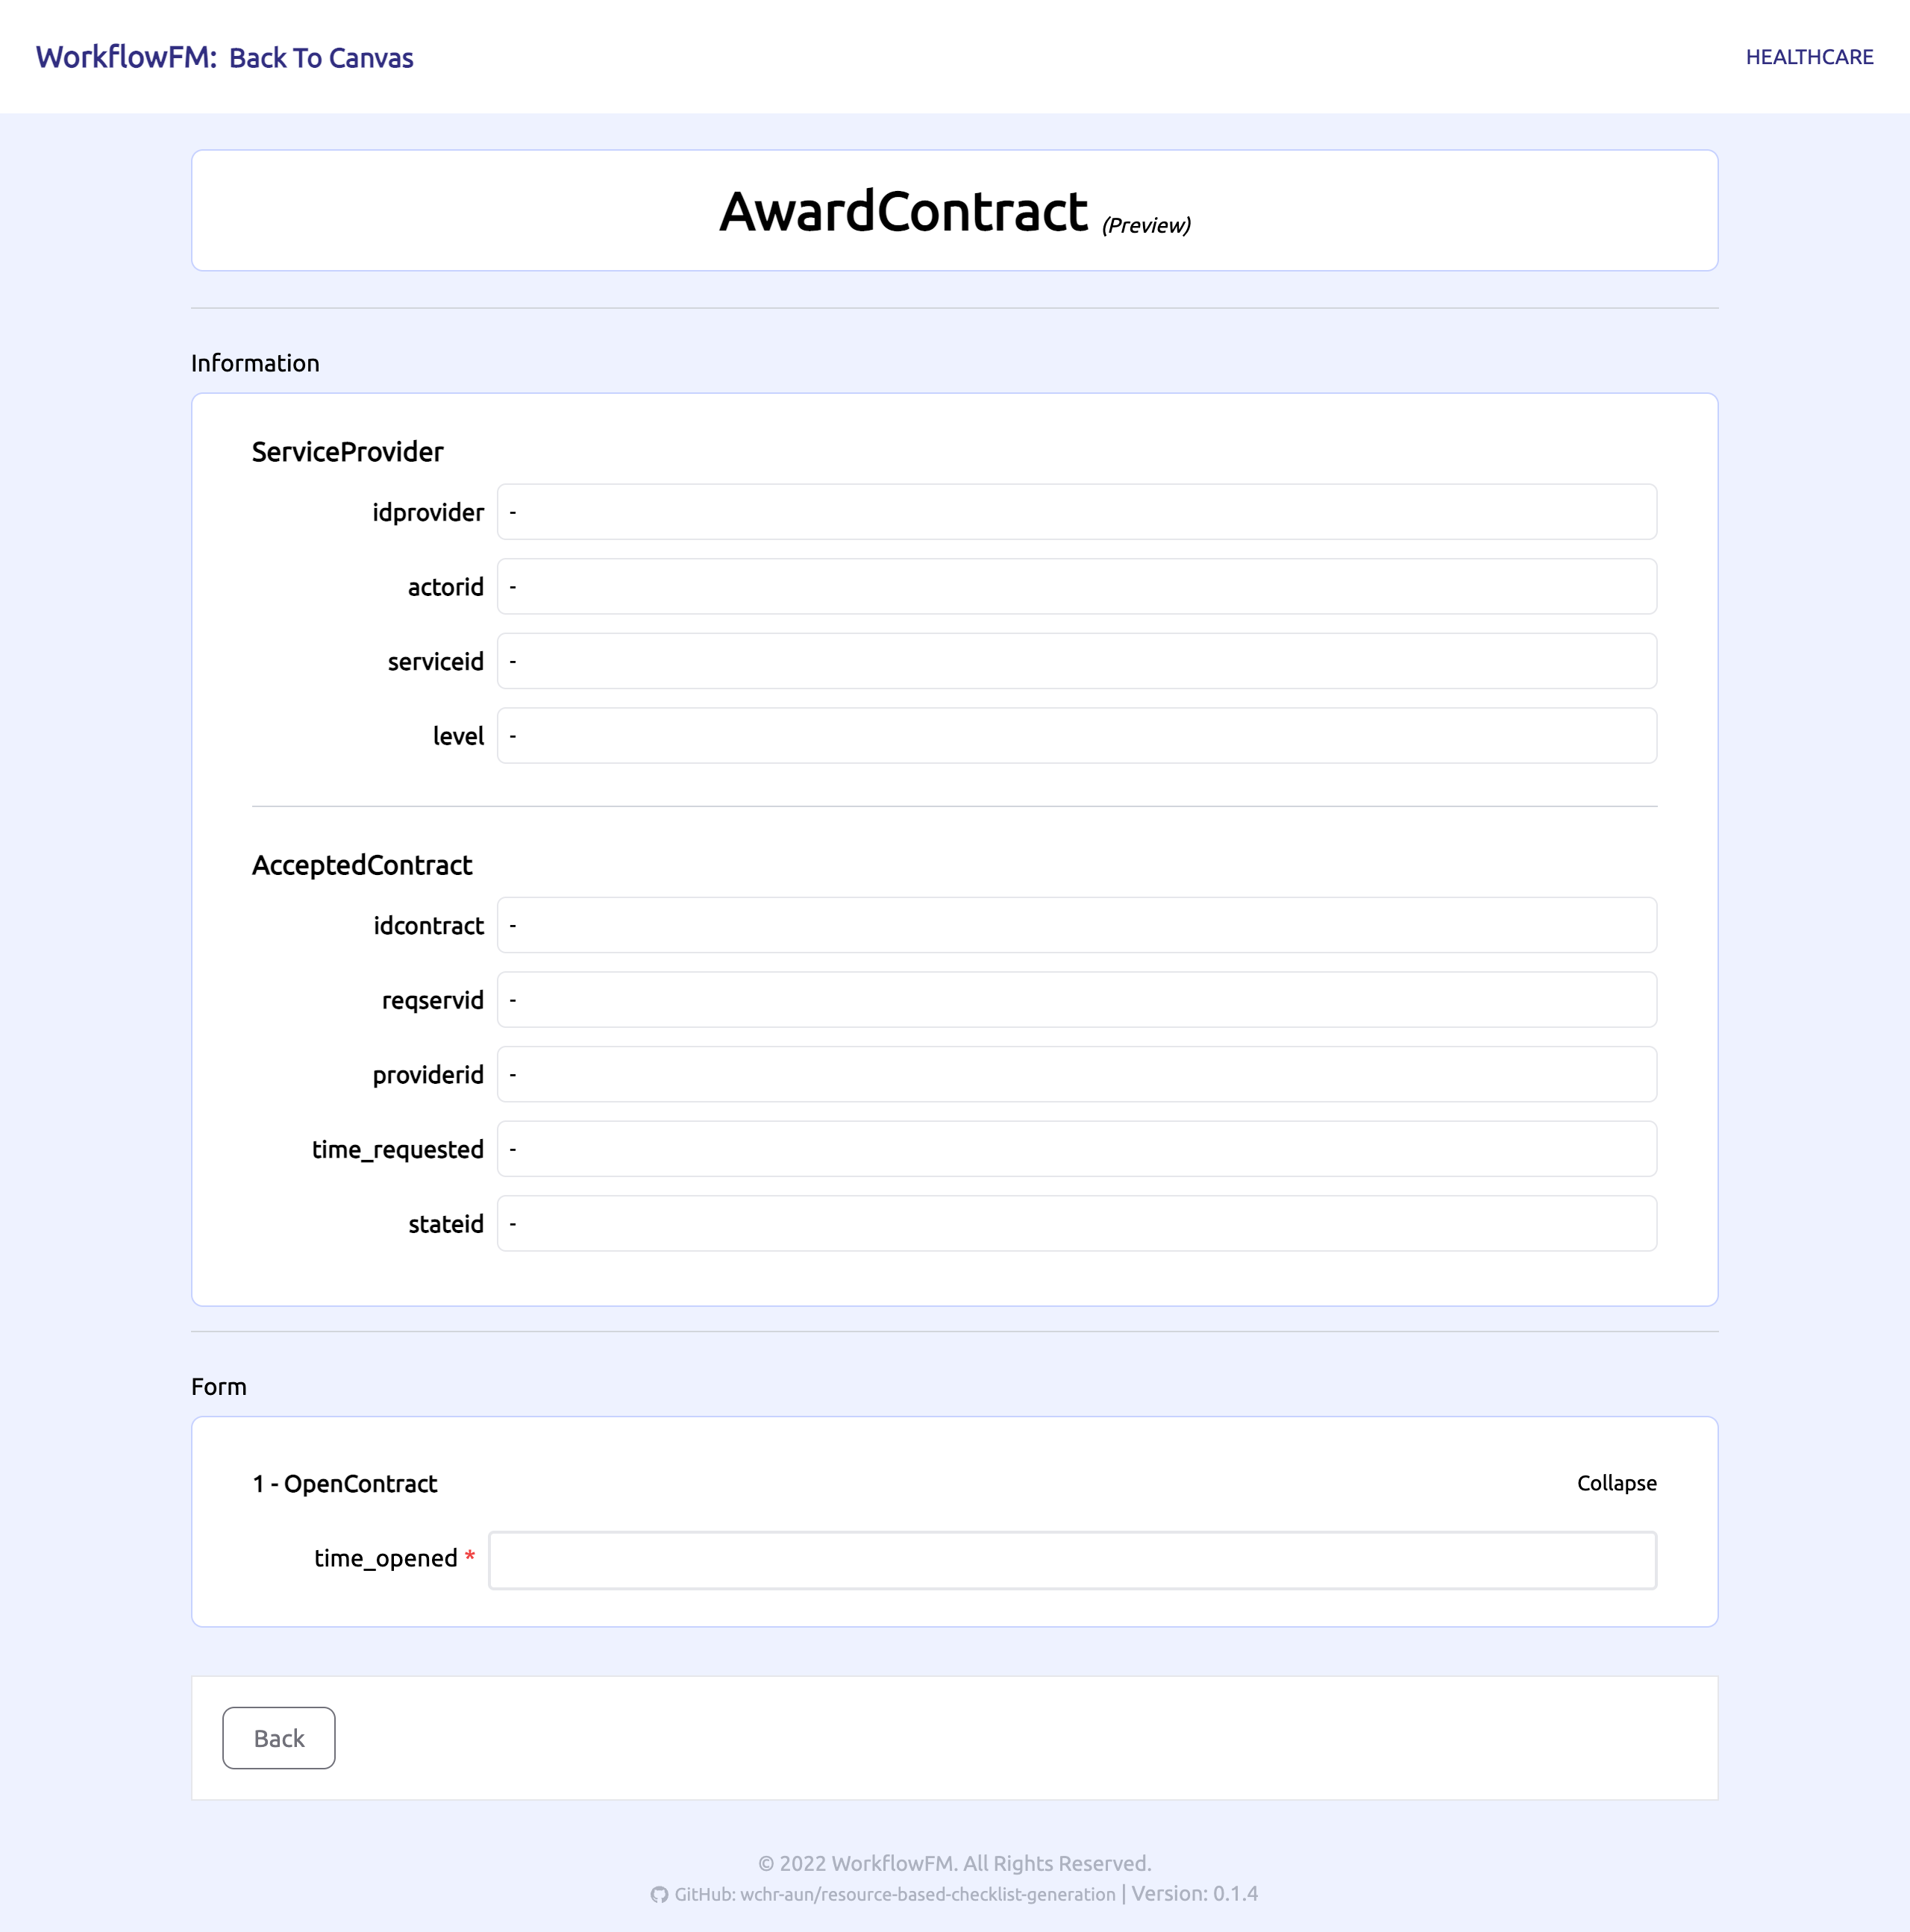
\includegraphics[width=0.9\linewidth]{overleaf/images/screens/preview_screen.png}
    \caption{Preview Screen}
    \label{fig:preview_screen}
\end{minipage}%
\begin{minipage}{.5\textwidth}
  \centering
    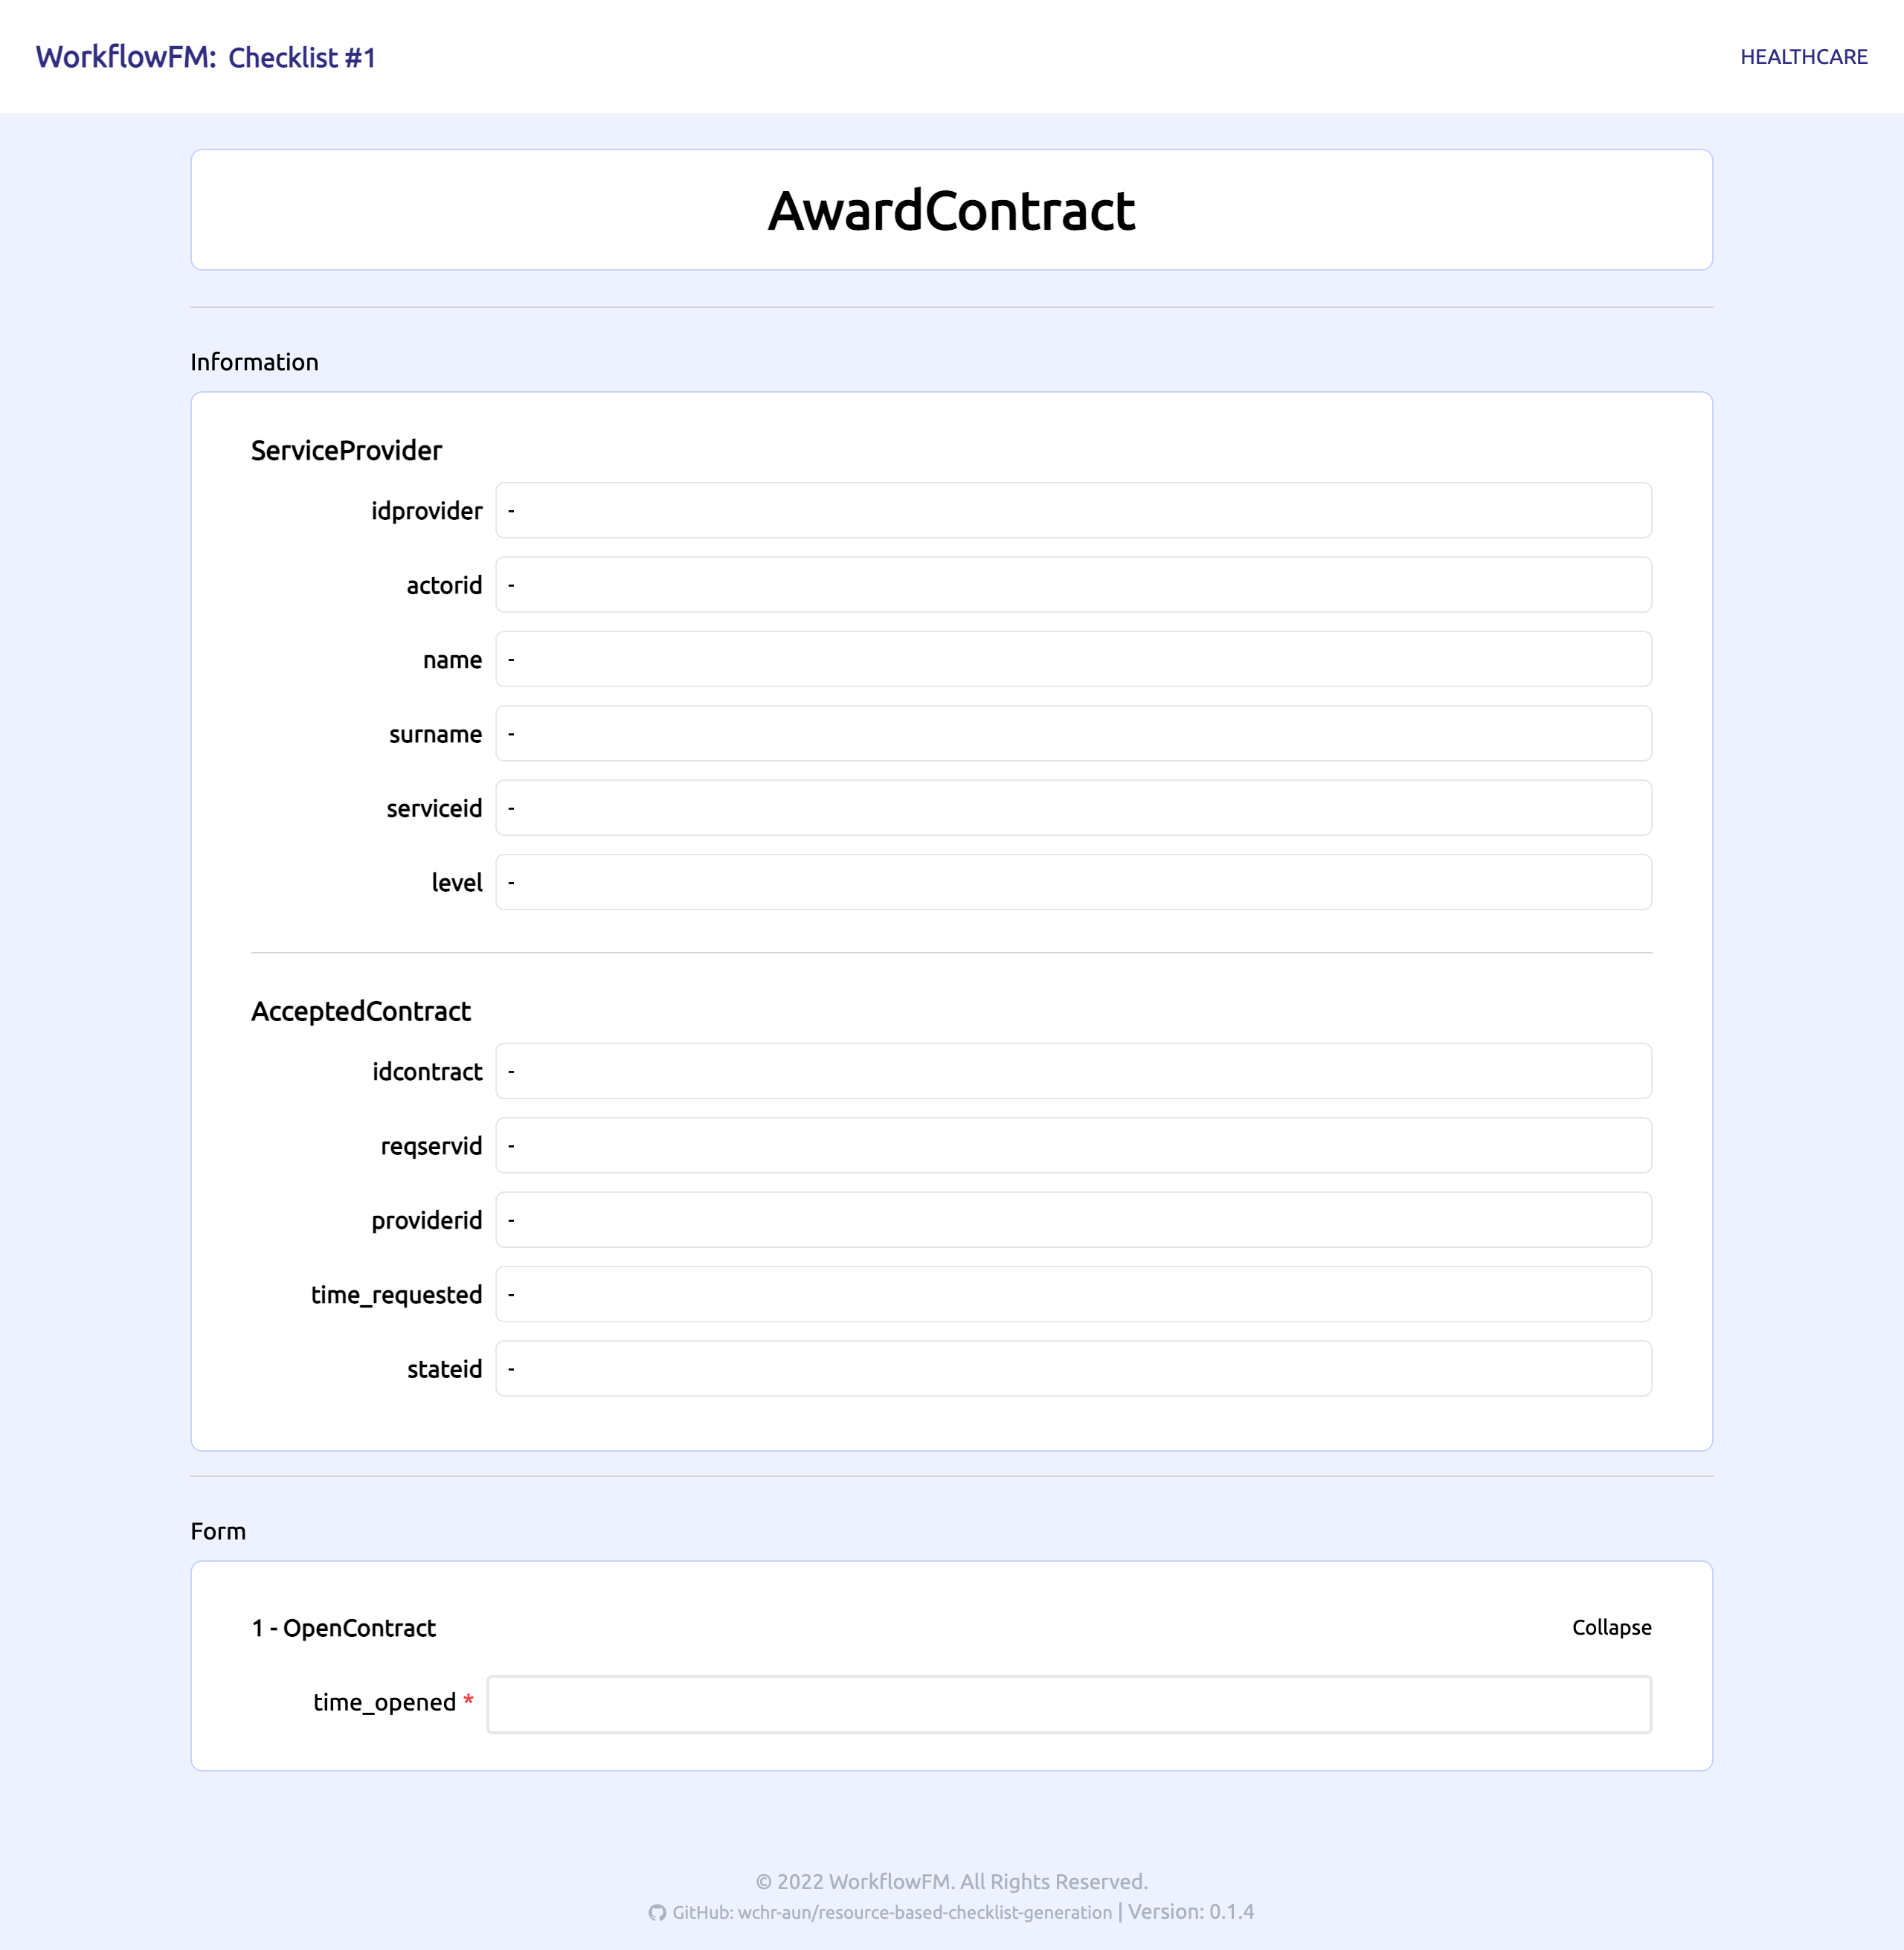
\includegraphics[width=0.9\linewidth]{overleaf/images/screens/view_checklist_screen.png}
    \caption{Checklist Screen}
    \label{fig:view_checklist_screen}
\end{minipage}
\end{figure}


\subsection{Checklist}
\label{im:view_checklist}

As discussed in the software's structure Section \ref{fig:software_structure}, this component only has one dynamic screen, as shown in Figure \ref{fig:view_checklist_screen}, which displays differently based on the selected template from the list on the main screen. Being able to view a saved template is part of the \textbf{Template Viewing} functionalities.


\section{Backend}
\label{im:backend}

The implementation of the backend is based on Section \ref{design:software_structure}, similar to the frontend. The backend is split into two components: template and dependency.
% The backend is hosted on Heroku\footnote{\href{https://msc-checklist-generation.herokuapp.com}{https://msc-checklist-generation.herokuapp.com}}.

% \subsection{Application Programming Interfaces}
% - workflow process to checklist template

% - get dependencies

% - get foreign tables/keys

% - saving template

% - retrieve finished templates


\subsection{Template}
\label{backend_template}
As stated in Section \ref{design:software_structure}, this component contains the template-related features, including CreateTemplate, SaveTemplate, GetTemplate, GetTemplates, and AutoGeneration.

\begin{itemize}
    \item \textbf{CreateTemplate} is a function that creates a checklist template based on the process's name, input and output.
    The templates follow the checklist template's structure \ref{checklist_strcuture} in Design. Initially, the process's name is set as the checklist's name, and the form components are set as empty. The input information, however, is queried from the entities of each leaf node of the process's input.
    Since the input of a workflow process is tree-structured, we need to use the Depth-first search algorithm \cite{dfs} to retrieve all the nodes inside the tree and flatten them into an array. Additionally, duplicated nodes need to be removed because they could exist in a different branch in the tree.
    
    Referring back to the functionality specification section \ref{functional_spec}, the \textbf{Template Creation} functionality is provided here.
    \item \textbf{SaveTemplate} is a function that disassembles and stores an incoming checklist template into the database.
    Since PostgreSQL cannot store tree-like data, templates need to be disassembled into four parts following the checklist template's models section \ref{checklist_models}.
    
    Referring back to the functionality specification section \ref{functional_spec}, the \textbf{Template Saving} functionality is provided here.
    \item \textbf{GetTemplate} is a function that allows the checklist screen (\ref{im:view_checklist}) to retrieve a checklist template given the id number of the template.
    Since templates are deconstructed in the SaveTemplate function, it is necessary to assemble parts in order to provide a correctly structured checklist template.
    
    Referring back to the functionality specification section \ref{functional_spec}, the \textbf{Template Viewing} functionality is provided here.
    \item \textbf{GetTemplates} is a function that returns the metadata (i.e. the name and the creation time) of most recent saved templates and displays as a list on the main screen (\ref{im:landing}).
    % This function does not have a direct connection to the functional specification, but it indirectly guides users to the checklist screen (\ref{im:view_checklist}) correctly.
    % \item \textbf{DeleteTemplate} is a function that deletes a checklist template given the id number of the template.
    
    \item \textbf{AutoGeneration} is an extended function on top of the \textbf{CreateTemplate} function that generates form components according to the process's output, as well as links of the dependencies based on the input's and output's entities.
    
    The algorithm to generate form components utilises the Depth-first search (DFS) algorithm \cite{dfs}, much like the \textbf{CreateTemplate} function, as part of it. The psudocode of the algorithm is illustrated in Appendix \ref{appendix:auto_gen_psudo}. To summarise, the psudocode is:
    
    \begin{enumerate}
        \item The algorithm starts with the DFS algorithm to go through each output node.
        \item If the current node is either a parallel or an optional, then create a header component that contains its children.
        \item If the current node is a leaf node:
        \begin{enumerate}
            \item Iterate over each field in the node's entity.
            \item Set the component type as a text box.
            \item Set the output dependency as the entity name.
            \item Set the output dependency field as the field in the entity.
            \item Set the input dependency and input dependency field based on the get input dependency function.
            \item Set the component children as empty.
        \end{enumerate}
        \item In the get input dependency function:
        \begin{enumerate}
            \item Retrieve the most frequent input dependency and input dependency field from existing templates in the database.
            \item If there is no existing template, look through the input's entities if there is a match. Else return the most frequent dependencies.
            \item If there is no match from the input's entities, then return empty. Else return the match.
        \end{enumerate}
    \end{enumerate}
    
    % To generate form components, it is necessary to use the Depth-first search algorithm \cite{dfs}, much like the \textbf{CreateTemplate} function, to go through each node in the output and construct a component based on them. The algorithm to construct a component is:
    
    % \begin{itemize}
    %     \item If the node is not a leaf node (being \verb!times! or \verb!plus!), then construct either a header or a tab component based on the node type (a header component for \verb!times! and a tab component \verb!plus!)
    %     \item If the node is a leaf node, then construct a header component with text boxes following fields in the node's entity.
    %     \begin{itemize}
    %         \item The output dependency is set to the entity's field.
    %         \item The input dependency is set to the entity's field of the input if it is the same field with the output's. Else empty.
    %         % empty as the default, but if they share the same entity's fields with the input's
    %     \end{itemize}
    % \end{itemize}
    
    With that said, this function is the \textbf{Auto Generation} functionality from the functionality specification section \ref{functional_spec}.
\end{itemize}


\subsection{Dependency}
\label{backend_dependency}
This component, as mentioned in section \ref{design:software_structure}, contains all the dependency-related features: QueryInputInformation and SuggestedQuery.
\begin{itemize}
    \item \textbf{QueryInputInformation} is a function that provides a list of possible entities in the database that the incoming entity's field is linked to regardless of the relation. This is a part of the \textbf{Input Information Query} functionalities that prepare the list to display on the frontend. For example, an entity called ``orders" contains \verb!order id!, \verb!customer id!, and \verb!total price! as its fields. The order id is linked to the transactions entity as a parent key, and the customer id is a foreign key to the customer entity. Given the example, this function will return the transactions entity for \verb!order id!, the customer entity for \verb!customer id!, and nothing for \verb!total price!.
    \item \textbf{SuggestedQuery} is a function that returns the most used group of input information fields in the database. This is a part of the \textbf{Query Suggestion} functionalities that retrieves the set of input information fields to display in the frontend. To retrieve the most used group from the database is as follows:
    \begin{enumerate}
        \item Group all the queried input information fields by the template.
        \item Count the amount of similar groups.
        \item Sort the groups descendingly.
        \item Return the first group.
    \end{enumerate}
    
\end{itemize}

% \subsection{Checklist}
% \subsection{Naive Queryable Field Suggestion}
% \subsection{Naive Dependency Suggestion}


\section{Testing}
Once we finished implementing both the frontend (\ref{im:frontend}) and the backend (\ref{im:backend}), we started testing the prototype with various examples that we had collected from the product owner. Though there were ten various examples, which can be seen in Appendex \ref{appendix:testing}, we only chose to present just two of them: a simple example and a complex example.

The easier example is the Award Contract process, as shown in Figure \ref{fig:AwardContract}. The Award Contract process is a process in which a clinician agrees to another member of the clinical staff to provide medical service on their behalf (i.e. delegating the task to someone else). The process contains the medical contract for the treatment (AcceptedContract); and delegated clinical staff (ServiceProvider) as the input and the same medical contract that has changed the status from ``accepted" to ``open" (OpenContract) as the output.

The more complex example is the Provide Service process, as shown in Figure \ref{fig:ProvideService}. This process is a process in which the doctor who is assigned to perform a healthcare service to either 1.) update the status of the service from ``pending" to ``completed" or 2.) inform about obstacles have occurred and are blocking any further progress. The process's inputs are the contract for the treatment (OpenContract) and the healthcare service in request (PendingHealthcareService). As for the output, it can either be 1.) an update of the healthcare servicefrom ``pending" to ``completed" (CompletedHealthcareService) or 2.) an notice of what obstacle is blocking the progress (Obstacle) and the exact same healthcare service (PendingHealthcareService).


\begin{figure}[ht!]
\centering
\begin{minipage}{.45\textwidth}
  \centering
    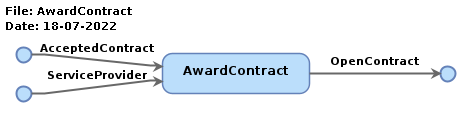
\includegraphics[width=0.9\linewidth]{overleaf/images/testing/AwardContract.png}
    \caption{Award Contract}
    \label{fig:AwardContract}
\end{minipage}%
\begin{minipage}{.55\textwidth}
  \centering
  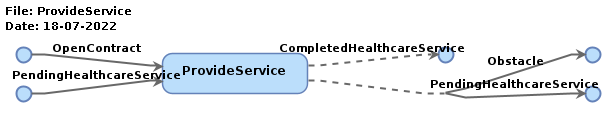
\includegraphics[width=0.9\textwidth]{overleaf/images/testing/ProvideService.png}
  \caption{Provide Service}
  \label{fig:ProvideService}
\end{minipage}
\end{figure}

Both examples were used to test against every functionality in the prototype, and both of them worked flawlessly. This is a good indicator that the prototype is working as intended.


\section{Challenges}

In this section, we will highlight two interesting challenges that we faced during the implementation. The first challenge is about the data structure. As mentioned in Section \ref{background:input_output}, the process's input and output are a tree-like structure. This leads to the use of a tree-like structure for the entire project because of the consistency and the ease of transforming data. However, a tree-like structure is complicated and takes some time to implement an algorithm such as the \textbf{AutoGeneration} in Section \ref{backend_template}. The Depth-first search (DFS) algorithm \cite{dfs} is used across both the frontend and the backend. Though it is not mentioned in Section \ref{im:frontend}, the frontend also needs to apply the DFS algorithm to render elements such as the form components that can contain children beneath.
This is why we use a tree-like structure in the frontend.

The second challenge is about computing statistical results. As discussed about the get input dependency function (in the \textbf{AutoGeneration}) and the \textbf{SuggestedQuery} in Section \ref{im:backend}, both features need to get statistical information from the existing templates in the database.
This is difficult because everything needs to be in one SQL query. This requires a lot of complicated operations in the query.
Technically, we could compute the statistics on the backend by dumping all templates into it.
However, it would require a lot of memories to do so. Thus we decided not to.

%  (the get input dependency function for the \textbf{AutoGeneration})

% \begin{itemize}
%     \item 
%     \item The suggestion and the input dependency linking within one sql query is hard
% \end{itemize}

% tree structure of workflowfm's processes, doing all suggestions within sql queries, design challenges (queryable input fields)
% http4s sucks-akka-http works
